\documentclass[12pt,a4paper]{article}

\usepackage[T1]{fontenc}
\usepackage[latin1]{inputenc}
\usepackage{graphicx}
\usepackage{upquote}

\begin{document}
\title{%
    \begin{minipage}\linewidth
        \centering\bfseries\sffamily
        PID : Packaging - Integration - Development 
        \vskip3pt
        \large An integrated software development process
        	\vskip3pt
        	\large Users Document
    \end{minipage}
}

\author{
	Robin Passama\\
	CNRS Research Engineer\\
	Robotic Department\\	
	LIRMM - UMR5506 - University Of Montpellier\\	
	\texttt{passama@lirmm.fr}}
\date{October 2013}

\maketitle

\bigskip
\bigskip
\bigskip
\bigskip
\bigskip
\bigskip

\begin{figure}
\center

\includegraphics[scale=0.7]{images/logos_officiels.png}
\end{figure}


\pagebreak

\part*{Introduction}
The main goal of this document is to provide a method that helps improving the overall quality of the code and applications produced by the robotics department of LIRMM. By improving the quality we aim at:
\begin{itemize}
\item simplifying the understanding and the modification of code produced by others.
\item simplifying the reuse of software components we develop.
\item pooling software developments between robotic teams.
\end{itemize}

To achieve this goal the Finding, Writing, Compiling, Testing, Version controlling and Documenting of the code are mandatory concerns. This document define in part 1, how the whole development process is organized, which tools are used and which concepts are handled. Then part 2 provides a detailed explanation of how PID is used and which processes it supports.

\pagebreak

\tableofcontents

\pagebreak

\part{Fundamentals}

The following subsections explain fundamentals that need to be understood to start working with the PID methodology. First of all, root concepts are:

\begin{itemize}

\item \textbf{package} : a package is the basic unit for code development, unit testing, source version controlling, deployment specification, documentation writing. A package provides some functional code that can be reused (libraries, executables, header files, scripts, etc.) and depends on other packages either for its compilation (static libraries, header files archives/folders) or for its runtime use (dynamic libraries, executables, script-like files). It can contains as well an entire huge software (e.g. operating system) as a very elementary piece of code (e.g. header files, a library, etc.).A package has two main different forms :
\begin{itemize}
\item a source form. In this form, the package is a git repository that contains the  package's source code. It is something "alive" that is continuously evolving along development process.
\item a binary form. In this form, the package is a collection of software artefacts (headers, configuration files, executables, libraries, documentation, etc.) deployed in a given place of a file system. It is something static (does not evolved) that is associated to a specific version of the package's source form. A binary package can be embedded into an archive in order to be easily retrieved and deployed on a file system.
\end{itemize}

\item \textbf{workspace}:  the workspace is the folder hierarchy in which the user develops source packages and deploys the binary packages he uses (third party or resulting from its own package deployment). The basic idea is to avoid to use system dependencies : every software artefact in the development process is then local and relative to the workspace, except of course artefacts bound to system dependencies. 

\item \textbf{package server} : a package server is a computer (accessible across the network) that hosts many packages (either source or binary). It centralizes the access to packages, and handles the rights of the users for each package. It is responsible of the global version control of packages. It can also provides tools to manage the development of packages it hosts (teams members, bugs and activities tracking/reports, wiki, version history and development branches, visualization, etc.).
\end{itemize}
 
The present document helps normalizing the development of packages inside workspace, and the way packages and workspaces are managed on development servers. As definition of concept and process is intrinsically bound to the concepts and process involved in the software tools used, the section first quickly present these tools. Then we define core concepts of the PID methodology based on those of the tools.
 
\section{Tooling}

For each development task in a package, a tool is used to achieve this task. To ease the portability of code, only \textbf{cross platforms} tools are used:
\begin{itemize}
\item \textbf{git} is used for the concurrent version control and patching of the code. It is also the tool used to deliver and retrieve the source code.
\item \textbf{cmake} is used to manage the build process, but also deployment and test.
\item \textbf{doxygen} is used to generate api documentation of source code.
\item \textbf{latex} is the preferred language to write documents, since it allows to version the full content of file (raw text and structure of the document), as opposed to binary formats like Microsoft Word or Libre-Office that are not well handled by git.
\end{itemize}

Other tools used, like the compiler/linker (e.g. gcc) used with cmake, or the ssh agent used with git, or even development environment (e.g. Xcode, Eclipse) interfaced with cmake, git and doxygen, are supposed to be native (i.e. specific to the OS used) and so adapted by the user depending on the platform he uses and his own preferences.

\section{Package}
\label{sec:Package}

The package is the basic working unit for developers. A package :
\begin{itemize}
\item contains the functional source code.
\item contains the tests source code.
\item contains version control information files.
\item contains the compilation files used to : build the source code and documentation, run tests, generate configuration files, install its resulting binary form in the workspace and generate an installable archive of its binary form.
\end{itemize}

The main idea is that a package is self-explanatory. It does not means it contains all code and artefacts it uses but it contains all information needed to satisfy its dependencies. In other words considering a given package, its installation process is done using this information and the information contained in its dependent packages.

One important concept when dealing with PID packages is the concept of \textbf{component} : it is a software artefact produced  by a package. It may be either:
\begin{itemize}
\item a \textbf{library} : this is a component that can be reused by developers to build other components. We define three types of libraries : \textbf{shared} (runtime or load-time linked library), \textbf{static} (link time only linked library) and \textbf{header} (compile time only "linked" library).
\item an \textbf{application} : this is a component for end-users or developers that define a runtime behaviour. We define three types of applications : application (made for end-user or developers when it is a runtime component), example (demonstrating how to use libraries) and test (used only internally to a package to test its other components).
\end{itemize}

\pagebreak

\subsection{Package Structure}
\label{sec:PackageStruct}

A Package is generically structured according to the folder hierarchy defined below:
\begin{itemize}
\item the root folder of the package has the \textbf{name of the package}. This folder is basically a git repository which allows to manage concurrent work and version control on a package's content.
\item the \textbf{.git} folder contains version control related information, automatically managed by the git tool.
\item the root \textbf{.gitignore} file is used to exclude from version control some artefacts like temporary files.
\item the \textbf{CMakeList.txt} file is used to describe how to build, install and test the whole package. It also contains meta-information on the package (authors and institutions, repository address, license, etc.).
\item the \textbf{build} folder contains results from build process and contains two subdirectories: \textbf{release} and \textbf{debug}. Each of them contains the hierarchy of files and artefacts generated by the compilation process.
\item the \textbf{src} folder contains sources files (.c/.cpp/.cc in C/C++) of libraries. Each subdirectory of \textbf{src} contains sources use to build one or more library and is itself hierarchically organized according to developers needs. Libraries provided by the package are defined by the CMakeList.txt file contained in the \textbf{src} folder.
\item the \textbf{include} folder contains interface description files, typically exported (i.e. installed) headers files (.h, .hpp, .hh) in C/C++. Hierarchical organization in this directory is the same as in \textbf{src}. Non exported headers are let in the \textbf{src} folder, as they are not considered as a part of the interface of the package.
\item the \textbf{apps} folder contains source files for applications, an application being an example of the usage of a library, a runtime component or a end-user software. Each subdirectory of \textbf{apps} contains sources for one or more built application and is hierarchically organized according to developers needs. Applications provided by the package are defined by the CMakeList.txt file contained in the \textbf{apps} folder.
\item the \textbf{test} folder contains source files for test units. Each subdirectory of \textbf{test} contains sources for one or more test unit. Custom test programs and running tests applied to the package are defined by the CMakeList.txt file contained in the \textbf{test} folder.
\item the \textbf{share} folder contains user written documents and some specific files used by the build process. Its contains different basic subdirectories :
\begin{itemize}
\item the \textbf{doxygen} folder contains a "default" Doxyfile.in file that is used by doxygen to generate API documentation. This file can be modified by the user to add additional information to the generated documentation. The folder can also contain additional resources (like images), hierarchically organized according to developers needs, used by doxygen to integrate additionnal information in the API documentation.
\item the \textbf{cmake} folder contains cmake scripts (notably find scripts) that the package uses to find external resources like libraries. This is the place used only for very specific resources for which no default cmake script is available.
\item the \textbf{config} folder contains configurations files used by libraries and applications/tests of the package.
\item the \textbf{doc} folder contains "hand-written" documents (e.g. README files, tutorials, design documents, etc.).
\end{itemize}
The \textbf{share} folder define a CMakeList.txt file that can be used to install resources of the \textbf{doc} and \textbf{config} folders.
\item the \textbf{license.txt} file contains the license that applies to the source code produced in the package. This file is generated by the build process.
\end{itemize}

\pagebreak

\subsection{Package repository}

Package repositories are GIT repositories, whose content is structured according to the previously defined pattern. GIT is used to version all text files used (C/C++ sources, cmake scripts, latex sources, etc.). Only source form of a package is a git repository not its binary forms.

\subsubsection{Version Numbers as GIT Tags}
\label{sec:versiontags}

A package is continuously evolving along time and git provide an internal version representation of this evolution. Nevertheless, this representation is so fine grained (each time a modification is committed) that it is not really understandable by persons not involved in the package development. That is why we need a version representation that can be either understandable by users and developers. These versions, called \textbf{release version} are defined according to a specific policy.

A \textbf{release version} can be viewed as a screen-shot of the git repository at a given time of package's life. It is associated to a number (called \textbf{release version number}) that is uniquely identifying the version. Technically, a version if represented as a \textbf{GIT tag} : a git tag memorizes a given state of the repository and is marked with a unique label that is used to retrieve this state. In our context the label of the git tag represents the release version number and the repository state pointed by the tag corresponds to the release version. The labelling of git tags representing release versions follows the pattern bellow:
\begin{itemize}
\item the release tags have the shape \texttt{vX.Y[.Z]}
\item \texttt{X} is the major version number (starts with value 0). Change of major version number indicates that the code is no more completely backward compatible with previous versions. In other words, the interface of the package (some of the headers files it contains) has been modify in such a way that some function have change or disappeared, or the behaviour/meaning of existing functions completely changed. While X is 0 the version is considered as pre-released and so is not ready for use by third party developers.
\item \texttt{Y} is the minor version number (starts with value 0). It indicates an improvement that is completely backward compatible with previous version with same major version number. In other words, the only a little change of existing behaviours occurred OR the interface of the package has been improved with new functionalities without breaking the way one use the older functionalities.
\item \texttt{Z} is the patch version (starts with value 0). It represents a simple bug fix or a security fix. A patch changes nothing to the interface (no new behaviour/functionality) and modify only in a minimal way the internal behaviour.
\end{itemize}

Each time a new version of a package is released, its version number must be incremented according to the previously defined rules and a corresponding git tag is created. Here are some examples:
\begin{itemize}
\item 0.1.0 is the first pre-released version of the package.
\item 0.Y.Z. are early development pre-released version of the package.
\item 1.0.0 is the first release of source code.
\item 1.2.0  is a release of source code backward compatible with version 1.0.0.
\item 1.2.5 is a release of source code of version 1.2.0 with 5 bug/security fixes.
\item 2.0.0 is a release that is no more backward compatible with 1.X.Y versions.
\end{itemize}

\subsubsection{Development process with GIT branches}
\label{sec:gitbranches}

GIT branches are used to organize the development workflow by registering "increments" made in the repository. Increments are modifications of the repository content, either source code, documentation, etc. A git repository can have many branches representing parallel development work. Most of time developers create branches to isolate the work they do on a specific concern as regard of the software development. This work is keep isolated from the work made on other concerns until developers think this is the good time to integrate (or discard) them. From time to time GIT branches are created, deleted, and merged. Merging consists in registering modifications made in two or more branches into a single branch.

As GIT branches can be used to represent any type of concern their understanding can quickly become a real problem. That is why their usage is constrained according to a predefined pattern inspired from successful branching models. This pattern defines what is the meaning of branches, what they are use for and the way they are created and merged :

\textbf{Main branches} (see in figure~\ref{fig:perm-branches}) have infinite lifetime and must always be usable : their last commit must point to a state in which the package is compilable and executable with unit tests successful.
\begin{itemize}
\item The \textbf{master} branch contains the source code that always reflects a production-ready state. This branch is used to \textbf{tag} the released stable source code with version numbers but also to tag important intermediate states of the repository that reflect the development made for demonstrations and publications. 
\item The \textbf{integration} branch contains the detailed history of all the modification that have been realized on the repository. The source code of HEAD (pointer on the current state of the repository) always reflects a state with the latest delivered development changes for the next release. This is where any automatic nightly builds are built from, if any.
\item When the source code in the \textbf{integration} branch reaches a stable point and is ready to be released, all of the changes should be merged back into \textbf{master} somehow and then tagged with an adequate release number.
\end{itemize}


\begin{figure}
\center
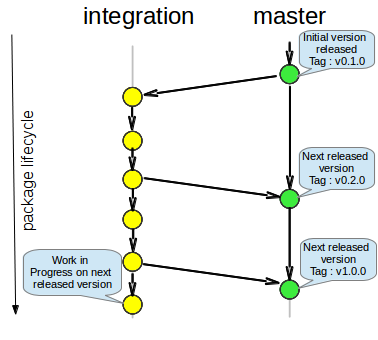
\includegraphics[scale=1]{images/permanent_branches.png}
\caption{Permanent branches of a package}
\label{fig:perm-branches}
\end{figure}

\begin{figure}
\center
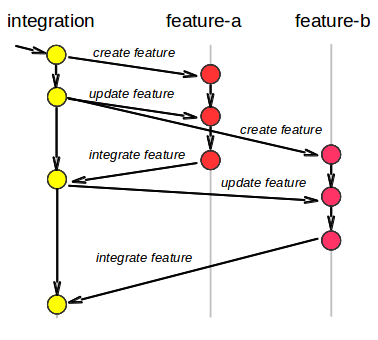
\includegraphics[scale=1]{images/feature_branching.png}
\caption{Relation between feature and integration branches}
\label{fig:feature-branches}
\end{figure}

\textbf{Supporting branches} are temporary branches, used to aid parallel development between team members, ease tracking of features and to assist in quickly fixing live production problems.
\begin{itemize}
\item \textbf{Features} branches (see figure ~\ref{fig:feature-branches}) are used to develop new features /address new topics for the upcoming or a distant future release. Each feature branch must branch from the \textbf{integration} branch. A feature branch exists as long as the feature is in development, but will be merged back into develop (to definitely add the new feature to the upcoming release) or discarded (in case of a disappointing experiment). During its lifetime a feature should be updated from time to time with the modifications contained in the \textbf{integration} branch (issued for instance from the integration of other features). Doing so, the final merge of the feature will be more easy as the state of the feature will be not to far, in terms of importance of modifications, from the state of the \textbf{integration} branch.
\item \textbf{Hotfixes} branches (see figure ~\ref{fig:hotfix-branches}) arise from the necessity to act immediately upon an undesired state of a released version. When a critical bug in a realease version must be resolved immediately, a hotfix branch may be branched off from the corresponding tag on the \textbf{master} branch that marks the production version. Hotfix branches are used to allow team members to continue their work (on the \textbf{integration} and \textbf{feature} branches), while another person is preparing a quick bug/security fix. When bugs are solved, the bug fix must be merged back into both \textbf{master} and \textbf{integration} branches. When merged the \textbf{master} branch is tagged with a new \textit{patch version number}.
\end{itemize}

\begin{figure}
\center
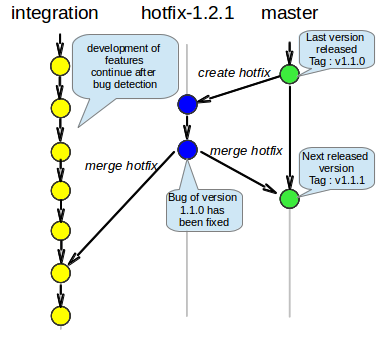
\includegraphics[scale=1]{images/hotfix_branching.png}
\caption{Relation between hotfix and integration/master branches}
\label{fig:hotfix-branches}
\end{figure}

\textbf{Naming Conventions:}
\begin{itemize}
\item a \textbf{feature} branch name starts with "feature-" and ends with the name of the feature (given by developer).
\linebreak example : \texttt{feature-newfunctionnality}
\item a \textbf{hotfix} branch name starts with "hotfix-" and ends with the new \textit{patch version} of the released version.
\linebreak example : \texttt{hotfix-1.2.1}
\end{itemize}

\subsubsection{Collaborative working with GIT repositories}
\label{sec:gitrepositories}

Now that the way the package is structured and is evolving the last part of this section consist in defining how people involved in the package's life cycle work together. The first concern is to define the \textbf{privileges} owned by these persons as regard of the repository usage. To do so we first define the three roles associated to each package:
\begin{itemize}
\item \textbf{users} are people using the package but not involved in its development.
\item \textbf{developers} are users involved in the development of a package.
\item \textbf{administrators} are developers with additional privileges, as they are considered as responsible of the package by users of the package.
\end{itemize}

Privileges associated to each role are managed inside the \textbf{package server} that hosts the package: 
\begin{itemize}
\item each package repository is associated to three \textit{groups}, each one representing a role previously defined. For example, for a package "a-pack" , there are groups "a-pack-users", "a-pack-developers" and "a-pack-administrators". Each group provides specific privileges on the package repository.
\item users registered inside the \textbf{package server} may be affected to one of these \textit{groups}. Doing so, these users obtain corresponding privileges on the package repository.
\item the repository can be set "public" so that anyone is considered as a user. In this case the users group may be not useful and can be let undefined.
\end{itemize}

\begin{figure}
\center
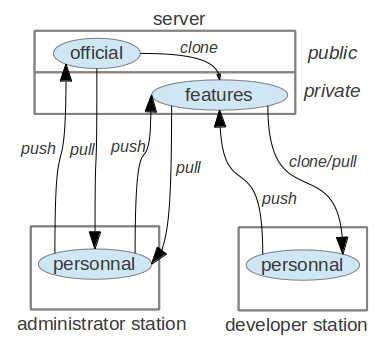
\includegraphics[scale=1]{images/collaborativework.png}
\caption{Collaboration between developers and repository}
\label{fig:collaborativeWork}
\end{figure}

The basic scheme for collaborative working between package developers is presented in figure~\ref{fig:collaborativeWork}. 
Given a package, this package has an \textbf{official GIT repository} that is deployed on a given \textbf{package server}. This repository is \textit{official} because it centralizes information of the package and is public, which means that all concerned people (team, laboratory or more generally anyone registered in the server) can access to it. The access in itself is restricted with respects to roles:
\begin{itemize}
\item registered \textbf{administrators} have read/write access on the official package.
\item all other registered \textbf{users} have read access.
\item unregistered people may have read access (i.e. open source repository).
\end{itemize}

During development, one or more \textbf{private repositories} of the package can be created by \textit{forking} the official repository. Depending on the official repository either only registered administrators (private package), developers (protected package), users (public package), or anyone (open package) can \textit{fork} the official repository. Then the creator in addition of the administrators of the official, become \textbf{administrators} of the private repository. Then they can register new \textbf{users} and \textbf{developers} for this repository, with following privileges:
\begin{itemize}
\item registered \textbf{administrators} and \textbf{developers} have read/write access.
\item registered \textbf{users} have read access.
\item unregistered people have no access.
\end{itemize}

These repositories help structuring the development process by grouping developers work around a common repository while not immediately impacting the official one. This lets the time to the \textbf{administrators} to check if everything is OK and that modifications can be merged back into the official repository. The main purpose when using \textbf{private repositories}, is to separate the work on the same package made by different groups. For instance, a PhD student working on its demos on one side and a team with external people working in a common research project on the other side.

Administrators of the official package are the only ones that can update the \textbf{official repository} with modifications made on private repositories. That is why they are responsible of \textit{version releasing} (see previous section): they check the work done by developers and decides if the code is stable enough to release it. Furthermore, if there are many private repositories of the same package they act as brokers of changes made in separate pools of developers.

\pagebreak

\section{Workspace}

The workspace is the place where developers work with packages (either those they develop or those they simply use). Technically, workspaces are local folder hierarchies in any station (server/demo/developers computers) that works with PID packages. A workspace is the place where packages repositories are created, developed and installed, and referenced given a predetermined pattern. As compared to classical "do as you wish" installation, the "workspace way of doing" as several advantages:
\begin{itemize}
\item there is a reference path in the deploy process in such a way that classifying and finding software artefacts is made easy.
\item there is no need to use system dependencies intensively for developed packages. As far as possible, every dependency should be satisfied by workspace content, except for system dependencies that cannot be packaged into workspace.
\item developers can handle many version of a package in the same build/execution environment, without risking to break OS dependencies. Furthermore they can used multiple versions of the same package in the same time.
\end{itemize}

\subsection{Workspace organization}

\subsubsection{Overview}
\label{sec:workspace}

A workspace is a folder (preferably named "workspace") with the following structure:
\begin{itemize}
\item the \textbf{.git} folder contains version control related information, managed by the git tool.

\item the \textbf{install} folder contains packages' binaries installed by the user. 
\item the \textbf{packages} folder contains all the packages developed by an author. Each sub-folder of \textbf{packages} is a local repository of a given package as presented previously.
\item the \textbf{external} folder contains all the external packages used by the installed package (source or binary). Each subdirectory corresponds to an external package, whose content is in turn completely undefined.
\item the \textbf{.gitignore} file is used to exclude  \textbf{install}, \textbf{packages} and \textbf{external} folders content from version control. This is mandatory since these folders content is supposed to be \textbf{ purely local a a user workstation}.
\item the \textbf{share} folder contains important files used to manage packages. The \textbf{docs} sub-folder contains documentation including the present document ; the \textbf{cmake} folder contains all scripts and data required to describe, build, install, deploy and configure packages: the \textbf{find} sub-folder contains cmake find script for commonly used external packages ; the \textbf{system} sub-folder contains generic scripts ; \textbf{patterns} contains cmake pattern files used ; \textbf{references} contains cmake script files with meta-information about available packages ; \textbf{licenses} contains cmake script files containing available license description; 
\end{itemize}

\subsubsection{Installing binary packages in the workspace}
\label{sec:workspaceInstall}

The \textbf{install} folder contains installed binary version(s) of any package used by a user. Each of its direct sub directories is a folder representing a given installed package, that itself contains :
\begin{itemize}
\item as many folders as there are concurrent binary versions of the package installed. The name of the version folder reflects the installed package version it contains (e.g. : 1.3.5 ; 1.2.0, etc.). Version folder can be also local (correspond to an install from a source package currently developed in the workspace), in such a case their name is of the form : own-0.2.5, own-1.0.0, etc.)
\item an \textbf{installers} folder that contains all installable binary archives with each archive that corresponds to a specific version, for a specific system (linux, mac), in a specific mode (release, debug).
\end{itemize}


Each version folder is organized according to the following structure:
\begin{itemize}
\item the \textbf{bin} folder contains all executables provided by the package, except tests, in both debug and release modes. In other words it contains the result of the compilation of its corresponding package repository \textbf{apps} folder.
\item the \textbf{include} folder contains the exported interfaces of libraries. Basically, its direct sub-folders are libraries' root folder hierarchically organized the same way as in the package repository \textbf{include} folder.
\item the \textbf{lib} folder contains libraries provided by the of the package in both debug and release modes.  In other words it contains the result of the compilation of its corresponding package repository \textbf{src} folder.
\item the \textbf{share} folder contains documents and scripts that are useful to the package users: the Use<Package><Version>.cmake file is a specific script file used to identify elements and dependencies of the binary package ; its \textbf{doc} sub-folder  contains API documentation generated by \textbf{doxygen} ; the \textbf{cmake} sub-folder contains cmake scripts files that are required to use the package, like find scripts used to configure external packages ; the \textbf{config} sub-folder contains installed element contained in the corresponding config folder of the package repository \textbf{src} folder ; the \textbf{doc} sub-folder contains "hand-written" documents installed with the package.
\item the \textbf{license.txt} file describes the license that applies to the software. This is a copy of the license file in package repository.
\end{itemize}

\subsection{Workspace repository}
\label{sec:workspaceRepository}

The \textbf{official workspace} is a git repository that can be modified only by \textbf{administrators} of the server. It contains cmake scripts used notably to:
\begin{itemize}
\item reference available packages (repositories and binary archives). Each time a new package is created it is referenced into the local workspace (by an administrator) and then changes in the official workspace are committed so that anyone can know the existence of this new package and can retrieve its hosting server. This does not mean that this person can use binary version or repository of this package, since this is bound to his access rights to the servers (at least one can know which person to call to get the rights).
\item provide available licenses description. These descriptions will be used in packages description.
\end{itemize}

The \textbf{official workspace} can be forked into \textbf{private workspaces}, exactly the same way as an \textbf{official package} (see figure~\ref{fig-collab}), to provide a common workspace for a team developing one or more packages at the same time. Once created new \textbf{users} and \textbf{developers} can be added to the private workspace repository. Private workspaces will be updated (by \textbf{developers} and \textbf{administrators}) with new references to packages, new licenses and new find scripts, while new packages are implemented. Then \textbf{official workspace} administrators can update its content, at any time, with the modifications made inside the private repository.

\pagebreak

\part{Usage}

This part of the document provides a detailed description on the usage of PID methodology's core concepts and tools. The first section describe how to use git tool to manage the collaborative work-flow. Second section describes how to use CMake tool to describe packages. Finally last section provides guidelines and advises to put in place good development practices.


\section{Work-flow management with git}

The purpose of this section is to define how to use the git tool to manage the whole life cycle of a project managed according to the principles of the PID methodology.

\subsection{Installing Workspace and Packages}

The first phase when starting development consists in installing a workspace on the local  station of a developer or administrator, and configuring it adequately. Figure~\ref{fig:install_workspace} provides a general overview of this operation.

\begin{figure}
\center
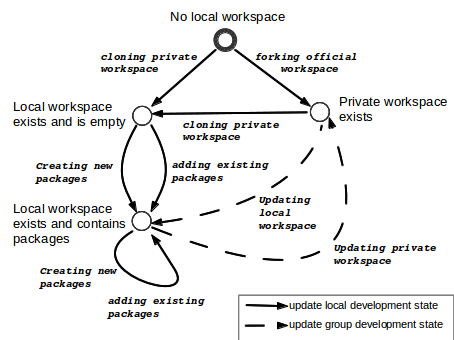
\includegraphics[scale=1]{images/installWorkspace.png}
\caption{State diagram showing how to deal with workspace}
\label{fig:install_workspace}
\end{figure}


\subsubsection{Getting a workspace}

The initial phase for any user is to \textbf{get a workspace on his local station}. More precisely a user needs to get a workspace repository that is connected to a \textbf{private workspace} (see section~\ref{sec:workspaceRepository}). This \textbf{private workspace} is used by a group of developers that work on same packages, for instance members of a same research team, members of a same research project, or even a single person for a PhD student whose work is isolated from the others. Only workspace administrators can create new private workspace repositories since their job is to know which persons can / have to work together.

This initial phase simply consists in either (see figure~\ref{fig:install_workspace}):
\begin{itemize}
\item if a \textbf{new group} is created for the developer:
\begin{enumerate}
\item  an administrator \textit{forks} the \textbf{official workspace repository} to get a \textbf{private workspace} on a server.
\item the developer \textit{clones} the \textbf{private workspace} in his local file system.
\end{enumerate}
\item if the developer will join an \textbf{existing group}:
\begin{enumerate}
\item  an administrator gives to him the privileges to access the \textbf{private workspace} of the group.
\item the developer \textit{clones} the \textbf{private workspace} in his local file system.
\end{enumerate}
\end{itemize}

Cloning and forking are similar operations, based on the clone action of the git tool like:
\begin{verbatim}
	git clone <account>@<official server>:workspace.git
\end{verbatim}
The main difference between both actions is where they take place. \textit{Cloning} is supposed to be done on local station of developers while \textit{Forking} is a clone action done in the official server. \textit{Forking} operation requires more actions like connecting to server and managing rights for developers that can access to the private repository: this can be easily achieved with Web based tool like GitHub or GitLab, but this is beyond the scope of this document.

When the local workspace repository has been cloned, the developer's workspace is empty, which means it only contains available licenses description in \textbf{licenses} folder, references to available packages in \textbf{references} folder but its \textbf{packages} and \textbf{install} folders are empty (see section~\ref{sec:workspace}).

\subsubsection{Adding packages to the workspace}

Since a \textbf{developer} is supposed to work on at least one package (but often more than one), he must add packages to its local workspace. To do so, he can create a new package and/or use existing packages.

\paragraph{Creating a new package:}
\begin{enumerate}
\item the developer creates a new \textbf{private package repository} on a \textbf{package server}. For the moment no \textbf{official package repository} exists for that package.
\item On his local station he then \textit{clones} the \textbf{private package repository} and initializes it the following way:
\begin{verbatim}
cd <workspace path>/packages
git clone <account>@<private server>:<new package>.git
cd <new package>
cp -R ../../share/patterns/package .
git commit -a -m "initialization of package done"
git tag -a v0.0.0 -m "creation of package"
git push origin master
git push origin tags/v0.0.0
git checkout -b integration master
git push origin integration
\end{verbatim}
\item then the developer starts working with its local and the private repositories (TODO add ref), he is the only person that can access it. At the beginning the package has a generic structure as in section~\ref{} but is empty: the first thing to do is to define package using CMakeList.txt files (see section~\ref{sec:useCMake}) and to add content (i.e. source code).
\item when the developer has reach a state in which the package can be delivered to the group he then:
\begin{enumerate}
\item generates/installs the \textbf{reference file} and the \textbf{find file} for that package using adequate CMake configuration (see section~\ref{sec:configCMake}): the \textbf{reference file} and the \textbf{find file} are respectively put is put into \textbf{references} and \textbf{find} folders of its local workspace (see section~\ref{sec:workspace}).
\item updates the \textbf{private workspace repository} of its group by doing:
\begin{verbatim}
cd <workspace path>
git add --all
git commit -m "adding new package : <package added>"
git push origin master
\end{verbatim}
\end{enumerate}
\end{enumerate}

\paragraph{Using existing packages:}
\begin{enumerate}
\item the \textbf{administrator} gives to the \textbf{developer} the adequate privileges on the used \textbf{private package repositories} (those developed by its group, or only part of them).
\item On his local station the \textbf{developer} then \textit{clones} the \textbf{private package repository}:
\begin{verbatim}
cd <workspace path>/packages
git clone <account>@<private server>:<used package>.git
\end{verbatim}
\item then the developer starts working with its local and the private repositories (TODO add ref).
\end{enumerate}
 
\textbf{Important remark:} all packages developed by a group must be \textbf{referenced} with the references files available in the \textbf{private workspace repository} of this group. Each package developed is itself connected to a given \textbf{private package repository} as explained in section~\ref{sec:gitrepositories}. Doing so each group work on an isolated development environment. Environments of groups are synchronized in two ways:
\begin{itemize}
\item \textbf{private package repositories} are updated with modifications made on \textbf{official package repositories} and reversely. These updates are completely managed by administrators who have the rights to modify \textbf{official package repositories}. This synchronization can be done progressively during packages development process.
\item \textbf{official workspace repository} is updated with modifications made on \textbf{private workspace repositories}. These updates are completely managed by administrators who have the rights to modify \textbf{official workspace repository}. This synchronization is mainly done when development process in a group has reached a stable state and after the first release of packages that have been created by a group.
\end{itemize}

\subsubsection{Installing other required packages in the workspace}

Whether a developer creates or use an existing package, this later can have dependencies with other packages and with system or external packages (see section~\ref{sec:rootCMakeDeps}). System dependencies are installed using standard install process provided by the OS (e.g. apt-get on Ubuntu/debian distributions) while external dependencies are installed "by hand". Package dependencies are installed using PID specific CMake procedure based on the \textbf{reference files}.

Each \textbf{reference file} of the workspace provide meta-information on a given package, notably the address of its git repository and addresses where to find binary package versions relocatable archives of this package (see section~\ref{sec:CMakeInstallBinary}). These informations are used to install adequate version of a required package at let two alternatives to install a package dependency:
\begin{itemize}
\item the git repository is accessible (at least in reading) by the developer and he can then clone and build it.
\item the adequate binary archives can be downloaded  by the developer and he can then directly install them.
\end{itemize}
In both cases, the process can be automatically managed by PID specific CMake scripts, which is the far most simple way. Otherwise the user can do this "by-hand", but this is beyond the scope of this document (i.e. reserved to expert users).

The only important thing to understand is the role of \textbf{reference files} and how they must be managed. In \textbf{private and local workspace repositories}, there is a set of \textbf{reference files that simply represent all available packages}. These reference files contain information on git repositories of packages, structured according to the following pattern:
\begin{itemize}
\item a reference file of a package that is not developed by the group contains the address of the \textbf{official package repository}. Members of the group don\textbf{'t have write access} to this repository and \textbf{may have read access or not}. It also contains addresses of downloadable binary package version relocatable archives whose access is generally open to all members of the robotic department or even sometime beyond (opened to partners, public access).
\item a reference file of a package that is developed by the group contains the address of the \textbf{private package repository}. Each time a member of the group \textit{forks} an \textbf{official package repository} into a \textbf{private package repository} he has to:
\begin{enumerate}
\item \textit{clone} the \textbf{private package repository} into his local workspace.
\item change the address of the package repository (official package repository address) with the address of the newly created \textbf{private package repository} (see section~\ref{sec:rootCMakeGeneral} and section~\ref{sec:PIDCMakefunctionsAPI_add_reference}).
\item generate the new reference file using PID specific CMake package configuration (see section~\ref{sec:configCMake}).
\item update the \textbf{private package repository}:
\begin{verbatim}
cd <workspace path>/packages/<new private package>
git checkout integration
git add CMakeList.txt
git commit -m "updating git address of the repository"
git push origin integration
\end{verbatim}
\item update the \textbf{private workspace repository} (whose references folder has been modified with an updated reference file for the package):
\begin{verbatim}
cd <workspace path>
git add share/cmake/references/Ref<package>.cmake
git commit -m "changing git repository address for <package>"
git push origin master
\end{verbatim}
\end{enumerate}
\end{itemize}

When done, installation of packages repositories for other members of the group will be quite simple and will target adequate \textbf{private package repository} (for whose members will have right to access in read/write). Only administrator will be responsible to avoid doing mistakes when merging \textbf{private package repositories} into \textbf{official package repositories} and \textbf{private workspace repositories} into \textbf{official workspace repository}. Their main task will be (1) to remove references to \textbf{private package repositories} in package CMakeList.txt files and (2) to merge adequately \textbf{reference files} from private and official repositories.

\subsection{Collaborative package development}

All \textbf{developers} only work around \textbf{private repositories} of packages, while \textbf{administrators} are responsible of the update of \textbf{official repositories} according to the changes done in private repositories. Most of developments in \textbf{private repositories} are made in \textbf{feature branches} and merged into the \textbf{integration branch} (see section~\ref{sec:gitbranches}).

\subsubsection{Handling feature branches}

\begin{itemize}
\item Creating a feature branch (derived from \textit{integration} branch):
beginning of the day):
\begin{verbatim}
git checkout -b <feature name> integration
\end{verbatim}
\item When starting modification of a feature (for instance at the beginning of the day):
\begin{verbatim}
git checkout feature-<feature name> 
// now working on <feature name> branch
git pull origin feature-<feature name>
// now <feature name> branch is up to date
\end{verbatim}
\item During development of a feature, developers need to frequently "save" their work locally:
\begin{verbatim}
git add <modified or new files>
git commit -m "<telling modifications>"
\end{verbatim}
\item When finishing modification of a feature (for instance at the end of the day or when important modifications have been finished and committed):
\begin{verbatim}
git pull origin feature-<feature name>
git pull origin integration
// update with evolutions of the integration branch
git push origin feature-<feature name>
\end{verbatim}
\end{itemize}

During development on a feature branch, a developer may need to test some ideas without disrupting the work of all people working on the feature. In that case, he can work with a \textbf{new local branch} forked from feature branch. Modifications in this branch stay always local to the developer station. Furthermore modification should not be too big, these branches are used to test some ideas or to do bug fixes, not for developing big features (this is the role of feature branches) !
\begin{itemize}
\item Creating a local branch for testing an idea:
\begin{verbatim}
git checkout feature-<feature name>
git pull origin feature-<feature name>
//=> solving potential conflicts and testing
git push origin feature-<feature name>
git checkout -b <idea> feature-<feature name>
\end{verbatim}
\item During development of the idea, frequently save the work locally:
\begin{verbatim}
git add <modified or new files>
git commit -m "<telling modifications>"
\end{verbatim}
\item When idea is OK and can be integrated to the feature:
\begin{verbatim}
git pull origin/feature-<feature name>
//=> solving potential conflicts and testing
git rebase origin/feature-<feature name>
git checkout feature-<feature name>
git merge <idea>
git branch -d <idea>
git push origin feature-<feature name>
\end{verbatim}
\item otherwise if the idea is not good:
\begin{verbatim}
git checkout feature-<feature name>
git branch -d <idea>
\end{verbatim}
\end{itemize}

\subsubsection{Integration of features}

During development process, features are integrated as soon as their development is finished and their tests are OK. Integration simply consists in merging feature branch into integration branch:
\begin{enumerate}
\item Merging the feature in the development branch (only developer responsible of the merge):
\begin{verbatim}
git checkout feature-<feature name>
git pull origin feature-<feature name>
//=> solving conflicts and testing, now feature is OK
git pull origin integration
//=> solving conflicts and testing, now feature ready to be merged
git checkout integration
git merge --no-ff feature-<feature name>
//=> solving conflicts and testing, now integration OK
\end{verbatim}
\item Deleting the feature branch (only developer responsible of the merge):
\begin{verbatim}
git push origin integration
git push origin --delete feature-<feature name>
\end{verbatim}
\item Updating local repositories after merge in the private repository (all developers of the repository) :
\begin{verbatim}
git remote prune origin
git branch -d feature-<feature name>
\end{verbatim}
\end{enumerate} 

\paragraph{Remarks:}
\begin{itemize}
\item The development of features is made in parallel and they are merged indirectly in the \textbf{integration} branch at the very end, one at a time: features don't synchronize until merge. This let the possibility to developers to change some parts of the API/structure without immediately impacting the work made on others features.
\item The best way is to first create an initial feature branch that puts in place the general basis of the package (API, basic class hierarchy, etc.). Then, when this feature has been merged in \textbf{integration} branch, parallel development into many feature branches can start.
\item When merging, the resolution of conflicts \textbf{must be realized in feature branch} to avoid any problem in the integration branch while conflicts resolution takes place.
\end{itemize}

\subsubsection{Releasing a Package Version}

Releasing package versions is the responsibility of administrators. It generally consists in merging \textbf{integration} branch into \textbf{master} branch and then tagging the result in master with a version number (see section~\ref{sec:versiontags}). 

\paragraph{Version tags handling} is made the following way:
\begin{itemize}
\item creating a version number (annotated tags):
\begin{verbatim}
git tag -a v1.2.3 -m"<small description of the version>"
git push origin tags/v1.2.3
\end{verbatim}
\item listing all available versions:
\begin{verbatim}
git tag -l 'v*'
\end{verbatim} 
\item showing the information of a given version: 
\begin{verbatim}
git show v<version number>
\end{verbatim} 
\item getting the released version in package history:
\begin{verbatim}
git checkout tags/v<version number>
\end{verbatim} 
\end{itemize}
It sis also possible to use tags during on \textbf{integration} branch, for instance to memorize code state matching demos or papers. Then use \texttt{p<journal or conf>-<date>-<author>} pattern tags for papers and \texttt{d<name of demo>-<date>-<author>} pattern tags for demos.

\paragraph{Administrator's repositories} are most of time more complex than simple developers ones as they reference the \textbf{official repository} and at least one \textbf{private repository}. Administrators must so manage multiple references to repositories:
\begin{itemize}
\item Creation of the local repository of a given package:
\begin{verbatim}
cd <path to workspace>/packages/
git clone <package official repository>
\end{verbatim}
\item Registering a \textbf{private repository} for a given package:
\begin{verbatim}
cd <path to workspace>/packages/<package>
git remote add <private repository name> <repository address>
\end{verbatim}
\item Getting the state of a private repository, without merging the result with administrator's local branches:
\begin{verbatim}
git fetch <private repository name>
\end{verbatim}
\begin{verbatim}
git remote rm <private repository name>
\end{verbatim}
\end{itemize}

The release process takes place into the \textbf{administrator}'s stations.
\begin{enumerate}
\item Update administrator's station with modifications contained in integration branch of private (named \texttt{private}) and official (named \texttt{origin} for administrators) repositories :
\begin{verbatim}
git checkout integration
git pull private integration
//=> solving conflicts and testing
git pull origin integration
//=> solving conflicts and testing, now ready to be merged
\end{verbatim}

\item Merging master and integration branches in local repository of administrator's station:
\begin{verbatim}
git checkout master
git pull private master
git pull origin master
//=> solving conflicts and testing
git merge --no-ff integration
//=> solving conflicts and testing, ready to be released
\end{verbatim}

\item Updating version number. Setting the adequate version number in the package's CMakeList.txt to get \texttt{<released version>}, rebuilding package and then:
\begin{verbatim}
git commit -a -m "Bumped version to <released version>"
git tag -a v<released version> -m"<description of version>"
\end{verbatim}

\item Updating official and private repositories:
\begin{verbatim}
git push origin integration
git push private integration
git push origin master
git push private master
git push origin tags/v<released version>
git push private tags/v<released version>
//=> updated branches and tags of private and official repositories
\end{verbatim}
\end{enumerate}

\subsubsection{Developing a hotfix}

Creating a hot fix is always made on demand of an administrator, but can be realized either by himself or a developer. The process is quite the same as for features: 
\begin{enumerate}
\item Creating the hotfix branch in the private repository, derived from version <old version>:
\begin{verbatim}
git checkout tags/v<old version>
git checkout -b hotfix-<new patch version>
\end{verbatim}
\item During the bug correction, committing locally:
\begin{verbatim}
git add <modified files>
git commit -m "<commit message>"
\end{verbatim}
\item Saving work in the private repository:
\begin{verbatim}
git push origin hotfix-<new patch version>
\end{verbatim}
\item Updating version number, when bug or security problems have been solved. Setting the adequate version number in the package's CMakeList.txt to get \texttt{<new patch version>}, rebuilding package and then:
\begin{verbatim}
git commit -a -m "Bumped version to <new patch version>"
git push origin hotfix-<new patch version>
\end{verbatim}
\item Merging hotfix branch with master:
\begin{verbatim}
git checkout master
git merge --no-ff hotfix-<new patch version>
git tag -a v<new patch version> -m"<description of version>"
git push origin master
git push origin tags/v<new patch version>
\end{verbatim}
\item Merging the bug correction with the integration branch:
\begin{verbatim}
git checkout integration
git merge --no-ff hotfix-<new patch version>
//=> solving conflicts and testing
git push origin integration
\end{verbatim}
\item Deleting hotfix branch on local and private repositories:
\begin{verbatim}
git branch -d hotfix-<new patch version>
git push origin --delete hotfix-<new patch version>
\end{verbatim}
\item Releasing the patch version in the official repository. This is the role of administrators that do that on their own station:
\begin{verbatim}
git fetch private
git checkout integration
git pull private/integration
//=> solving conflicts and testing
git push origin integration

git checkout master
git pull private/master
git push origin master
git push origin tags/v<new patch version>
\end{verbatim}
\end{enumerate}

\pagebreak

\section{Package development with CMake}
\label{sec:useCMake}

When developing a package one need to handle information such as:
\begin{itemize}
\item \textit{meta-information}: who is involved in its development ? what is its general purpose ? where to find this package on the network ? what is the license of the code ? etc.
\item \textit{build-related information}: what are the components provided by the package and how to compile/link them from source code ?  How components are tested ? what is the version of the package ? what are its functional dependencies ?
\item \textit{functional information}: this is the source code of the components and other associated files like configuration files if any required.
\end{itemize}

The whole package development is organized and described with cmake, and the CMakeList.txt files used contain the whole \textit{meta-information} and \textit{build-related information} used by the package. Each package contains several CMakeList.txt files:
\begin{itemize}
\item the root CMakeList.txt file (direct leaf of the package source repository, see section~\ref{sec:PackageStruct}) is used to define \textit{meta-information} and \textit{dependencies} of the package.
\item the CMakeList.txt file contained in the \textbf{src} folder defines the \textbf{library components} (see section~\ref{sec:Package}).
\item the CMakeList.txt file contained in the \textbf{apps} folder defines the \textbf{application components} (see section~\ref{sec:Package}).
\item the CMakeList.txt file contained in the \textbf{test} folder defines the \textbf{test components} (see section~\ref{sec:Package}) and running tests (using these components or others).
\item the CMakeList.txt file contained in the \textbf{share} folder defines additional files to install, like configuration files used by libraries and/or applications (if any), documents, etc.
\end{itemize}

Each of these CMakeList.txt files must follow a predefined pattern. This pattern is mainly influenced by the use of PID specific CMake functions. The following subsections present examples on how to use these functions together with more classical CMake code in order to completely define a PID package.

\subsection{Package's root CMakeList.txt file}
\label{sec:rootCMake}

\subsubsection{General Meta-Information}
\label{sec:rootCMakeGeneral}

Let's suppose we define a package with the name "the-testpack-b", its root CMakeList.txt file could look like this.

\begin{verbatim}
PROJECT(the-testpack-b)
CMAKE_MINIMUM_REQUIRED(VERSION 2.8.11)
set(WORKSPACE_DIR ${CMAKE_SOURCE_DIR}/../.. CACHE PATH "root of 
the packages workspace directory")
list(APPEND CMAKE_MODULE_PATH ${WORKSPACE_DIR}/share/cmake/system) 
# using generic scripts/modules of the workspace
include(Package_Definition)

declare_PID_Package(	
    AUTHOR      Robin Passama 
    INSTITUTION LIRMM 
    YEAR        2013 
    LICENSE     CeCILL
    ADDRESS     git@idh.lirmm.fr:perso/passama/the-testpack-b.git
    DESCRIPTION 	test package B for PID
)

set_PID_Package_Version(1 1)

# adding some binary packages references
add_PID_Package_Reference(
    BINARY VERSION 0 1 0 SYSTEM linux 
    URL 	
    http://lirmm.lirmm.fr/FileX/get?auto=1&k=rfYTf1gkpI5XtEpQWVA		
    http://lirmm.lirmm.fr/FileX/get?auto=1&k=oMyg4JVeeKYWpqwEFxE
)

add_PID_Package_Reference(	
    BINARY VERSION 1 1 SYSTEM linux 
    URL 
    http://lirmm.lirmm.fr/FileX/get?auto=1&k=DYt2j35Kw8ozOgHfoVA
    http://lirmm.lirmm.fr/FileX/get?auto=1&k=zEx02N4KWfzDWPTxiO
)
\end{verbatim}

Exactly as in any CMake project, the CMake package is define with the PROJECT keyword. The project's name \textbf{is the name of the package root folder} (and so the name of the repository). The remaining lines until the \texttt{declare\_PID\_Package} macro call must be let \textbf{unchanged} (initialization of the PID specific cmake scripting system).

Then comes the \texttt{declare\_PID\_Package} macro, which is mandatory. This macro defines general meta-information on the package, and should not change a lot during package life cycle: 
\begin{itemize}
\item the main author (AUTHOR keyword) and its institution (INSTITUTION optional keyword), considered as the maintainer of the package. The main author is an \textbf{administrator} of the package (see section~\ref{sec:gitrepositories}).
\item the YEAR field helps defining the package's life cycle range. For instance one can input a field such as "2009-2013".
\item the LICENSE field is used to specify the license that applies to the code. This license must be defined in the workspace (see section ~\ref{sec:workspace}) in the form of a \textbf{cmake script license file}.
\item the ADDRESS field is used to specify the address of the \textbf{official GIT repository} of the package (see section~\ref{sec:gitrepositories}).
\item the field DESCRIPTION must be filled with a short description of the package usage/utility.
\end{itemize}
~\\

Then the user fill other meta-informations that evolve during project life cycle:
\begin{itemize}
\item the \texttt{set\_PID\_Package\_Version} function is used to set the currently developed version of the package. It take at least a MAJOR and MINOR numbers and optionally a PATCH number as arguments (default value for PATCH number is 0). The version number thus follows the same pattern as git \textbf{release versions}. Before a version is released with a git tag (see section~\ref{sec:versiontags}) this version number must be set adequately so that git tag matches cmake package version. Generally, the best way to do is set the version number used in the CMakeList.txt with the number of the next version to release.
\item the \texttt{add\_PID\_Package\_Reference} function is used to register a downloadable binary version of the package. The VERSION keyword specify the version with MAJOR MINOR PATCH numbers. The SYSTEM keyword specifies the target operating system for which the binaries have been built. The two addresses after the URL keyword specify where the binary package version can be downloaded either in release (first address) and debug (second address) modes.
\end{itemize}

\subsubsection{Dependencies with other packages}
\label{sec:rootCMakeDeps}

The last part of the root CMakeList.txt is used to manage dependencies between the current package and other packages it depends on. It could look like this:

\begin{verbatim}
# finding used packages
find_package (Boost REQUIRED)
find_package (the-testpack-a 1.0 REQUIRED lib-b-sh lib-x)

# declare a dependency over Boost (by default boost root is the 
# /usr system install dir)
if(Boost_DIR-NOTFOUND)
     set(BOOST_ROOT /usr)
endif()
declare_PID_Package_Dependency(PACKAGE Boost EXTERNAL 
${BOOST_ROOT} VERSION "${Boost_MAJOR_VERSION}.
${Boost_MINOR_VERSION}.${Boost_SUBMINOR_VERSION}")

#declare a dependency over the-testpack-a PID package
declare_PID_Package_Dependency (
                PACKAGE the-testpack-a
                PID VERSION 1 0 
                COMPONENTS lib-b-sh lib-x)
                
build_PID_Package()
\end{verbatim}

The \texttt{find\_package} function is a standard cmake function used to find and configure other packages. In the example, we search for a package named "the-testpack-a" (that is also a PID package) with version compatible with 1.0 (for PID packages compatibility as the same meaning as in section~\ref{sec:versiontags}, otherwise the meaning is package dependent). The package is REQUIRED meaning that it must be found.  We specifically require the \textbf{components} named "lib-b-sh" and "lib-x". As experienced CMake users may notice there is no difference in the usage of the \texttt{find\_package} function as regard of its standard use. 

Then PID development process imposes to declare dependencies of the current package. Indeed this is not because you try to find other package that you will use them, even if obviously this assumption will be right most of time. A dependency simply means that components of the package are using components from other packages (see section~\ref{sec:Package} to understand what is a component). For instance, the current package uses the package "the-testpack-a" with minimum version 1.0. To make this declaration possible PID provides the \texttt{declare\_PID\_Package\_Dependency} function. This function can be used in two different ways:
\begin{itemize}
\item it is used to specify a dependency to an \textbf{external package} (using the keyword EXTERNAL after the package name). An external package is just a \textit{reference} associated to a path that points to the root folder of a \textbf{NON PID} package. This reference will be used later when defining components. A version information can be appended but is not used. A good way to do is to install external package into the \textbf{external} folder of the workspace, when possible, so that they will be managed by PID in a easier way. External package are packages installed by hand by the user in his file system, either in system or add-hoc folders. For packages that are supposed to be part of the operating system, there is no need to specify the dependency since this dependency is satisfied "by default" by the system.
\item it is used to specify a dependency to a PID package (using PID keyword). Then version and component requirement informations can be used exactly as in the example. Relationship between PID packages are stronger since their discovering/install configuration will be done automatically.
\end{itemize}

Finally, the CMakeList.txt file call the \texttt{build\_PID\_Package} function. This line is mandatory in order to allow the build of the package: compilation, installation, deployment, API doc generation, etc. Without this call, the CMake process would simply do nothing.

\subsubsection{Dealing with conditional dependencies}
\label{sec:rootCMakeComplexDeps}

The previous example is quite simple since it directly deals with \textbf{required} dependencies. Nevertheless, when using cmake one sometimes have to deal with \textbf{conditional dependencies}. Indeed, \textbf{conditional dependencies} allow to configure the build according to the OS requirements or to the configuration of user's station. This conditional dependencies are managed according to the following pattern (or a derivative from this solution):
\begin{verbatim}
find_package(the-testpack-a)
if(the-testpack-a_FOUND)
    set(USE_the-testpack-a TRUE CACHE INTERNAL "" FORCE)
     declare_PID_Package_Dependency (PACKAGE the-testpack-a
                PID VERSION 1 0 COMPONENTS lib-b-sh lib-x)
else()
    set(USE_the-testpack-a FALSE CACHE INTERNAL "" FORCE)
    find_package(the-testpack-x)
    if(the-testpack-x_FOUND)
       set(USE-the_testpack-x TRUE CACHE INTERNAL "" FORCE)
       declare_PID_Package_Dependency (PACKAGE the-testpack-x
                PID VERSION 1 3 COMPONENTS lib-any)
    else()
       set(USE-the_testpack-x FALSE CACHE INTERNAL "" FORCE)
       MESSAGE("alternative system dependency not satisfied. 
       Install/select either the-testpack-a or the-testpack-x")
       return()       
    endif()
endif()
\end{verbatim}

Conditional dependencies is used to describe dependencies that are optional or to describe an alternative requirement when multiple different packages can be used for the same purpose. This later case is shown in the previous code. Defining such conditional dependencies is made using classical CMake mechanism (using \texttt{find\_package} and \texttt{option}/\texttt{set} commands) is combination with the \texttt{declare\_PID\_Package\_Dependency} function previously explained. In the previous example, there is an implicit priority in the usage of required packages: "the-testpack-a" will be used prior to "the-testpack-x" if it is found. The CMakeList.txt file can also use the \texttt{option} command to let the user select its preferred package. The only mandatory descriptive elements are:
\begin{itemize}
\item if a package is to be used, \textbf{whether it has been previously found or not}, then the \texttt{declare\_PID\_Package\_Dependency} function \textbf{must be called} to tell to PID system which package (PID or external) is required.
\item Each possibly used package must be bound to a CMake \textbf{variable that indicates if the package is really used or not}. For instance see the variable \texttt{USE\_the-testpack-a}. These variables will be used later, when declaring components, to know how to configure component dependencies according to required packages.
\end{itemize}

\subsection{Defining Library components}
\label{sec:libCMake}

Once package dependencies have been defined, the package developers can then define components of the package and their relationship with these dependencies. Most common components are library components : they are used by developers to define reusable functionalities. All libraries are defined in the CMakeList.txt file contained in the \textbf{src} folder of the package repository.

PID defines three types of libraries, matching the three classical  types available in C/C++. It provides a systematic way to define these libraries and automate their use, avoiding the user to know precisely how to deal with each type and their relative properties. Following subsections explain how to declare each of these types. These definitions rely on cmake functions provided by PID: \texttt{declare\_PID\_Component} and \texttt{declare\_PID\_Component\_Dependency} (see appendix~\ref{sec:PIDCMakefunctionsAPI}).

\subsubsection{Header libraries}
\label{sec:libCMakeHeader}

Header libraries are not compiled to produce a binary object. They are just made of a set of header files. This kind of library used is often used for template libraries definitions, for instance the Boost library. Such a library is never used at link time (never linked to another library or executable using a linker) but only at compile time (when including header files). The definition of a header lib should look like:
\begin{verbatim}

declare_PID_Component(HEADER_LIB NAME lib-y DIRECTORY lib_y)
declare_PID_Component_Dependency(COMPONENT lib-y 
               EXPORT DEPEND lib-x PACKAGE the-testpack-a
               EXPORTED_DEFINITIONS USE_EXTERNAL_LIB_X)

\end{verbatim}

The first thing to do is to declare the header library by using the function \texttt{declare\_PID\_Component}:
\begin{itemize}
\item the HEADER\_LIB keyword is used to declare a header library.
\item the NAME keyword is used to define the identifier of the component in PID, whose unicity must be preserved. In the example the name is "lib-y".
\item the DIRECTORY keyword is used to say in which sub-directory of the \textbf{include} folder the header files are found, in the example the "lib\_y" sub-folder. The direct consequence is that all headers of a given library \textbf{must be placed in a unique folder}.
\end{itemize}
 
Then, depending on the library content, some dependencies can be attached to the library, using \texttt{declare\_PID\_Component\_Dependency}. Indeed a header library can depend on other libraries, either header, static or shared:
\begin{itemize}
\item the COMPONENT keyword is used to specify for which component a dependency is defined, in the example the previously defined "lib-y" header library.
\item the EXPORT keyword specifies that the lib-y component export the required dependency. Exporting means that the reference to the required component is defined in the interface of the library. Since a header lib is only made of an interface, \textbf{it must export each of its dependencies}.
\item the DEPEND and PACKAGE keywords are used to specify the dependency: here the lib-y header library depends on the component "lib-x" of the PID package "the-testpack-a". Declaring an external or system dependency or even an internal dependency is slightly, but follows the same logic, see appendix~\ref{sec:PIDCMakefunctionsAPI}.
\item the EXPORTED\_DEFINITIONS is used to specify values of C preprocessor definitions that are exported by the library. In the example the exported definition is \texttt{USE\_EXTERNAL\_LIB\_X}. exported definition are used by components that will use lib-y to configure its code adequately. Since a header lib is only made of an interface, all its definitions must be exported and it can have no internal definitions.
\end{itemize}

On interesting property of PID is to be able to declare different components from the same code. For instance:
\begin{verbatim}

declare_PID_Component(HEADER_LIB NAME lib-y-bis DIRECTORY lib_y
                      EXPORTED_DEFINITIONS NUSE_EXTERNAL_LIB_X)

\end{verbatim}

In this later example, a new component named "lib-y-bis" is created from the same source code contained in the lib\_y folder. The differences with the previous component are that the "lib-y-bis" has no dependencies and it undefines (using N in front of the preprocessor definition) the definition \texttt{USE\_EXTERNAL\_LIB\_X}. This is useful to declare many alternatives from the same code.

\subsubsection{Static libraries}
\label{sec:libCMakeStatic}

Static libraries are binary archives that define some functionalities. A static library is made of:
\begin{itemize}
\item a set of header files that define its interface (i.e. what is available for library users).
\item a set of (compiled) binary objects that implement its behaviour.
\end{itemize}
Its interface is used at compile time (when its header are included) and its contained objects are linked to executables and shared libraries at link time, so they no more exist at run time. The definition of a static lib should look like:

\begin{verbatim}

declare_PID_Component(STATIC_LIB NAME lib-c-st DIRECTORY lib_c
                  INTERNAL DEFINITIONS NA_VERY_SPECIFIC_IMPLEM)
declare_PID_Component_Dependency(COMPONENT lib-c-st
                  EXTERNAL Boost INCLUDE_DIRS <Boost>/include)
declare_PID_Component_Dependency(COMPONENT lib-c-st 
                  EXPORT DEPEND lib-y-bis)

\end{verbatim}

As for any component, the first thing to do is to declare by using the function \texttt{declare\_PID\_Component}:
\begin{itemize}
\item the STATIC\_LIB keyword is used to declare a static library.
\item the NAME keyword is used to define the identifier of the of the static library, "lib-c-st" in the example.
\item the DIRECTORY keyword is used to say in which sub-directory of the \textbf{include} folder the header files of the static library are found, in the example the "lib\_c" sub-folder. The \textbf{same folder name} is used to specify in which subdirectory of the \textbf{src} folder the source and non-public header files of the library are found. For a same library, this constraints the user to use same folder names between \textbf{include} and \textbf{src} directories.
\item the INTERNAL DEFINITIONS is used to specify definitions that affect only the implementation (i.e. that is not used in any header file of the library). In the example the "lib-c-st" undefines the preprocessor definition A\_VERY\_SPECIFIC\_IMPLEM .
\end{itemize}

As readers can notice, the declaration is quite the same as for header libraries. Note also that static libraries can define exported definitions (as header libraries) for those which are used in their header files. The declaration of dependencies also follows the exact same pattern. In the example:
\begin{itemize}
\item "lib-c-st" static library is using an external package named "Boost". As boost is a pure header library it only needs to specify where to find its header files, using the INCLUDE\_DIRS keyword. The include path specified is relative to the Boost package root folder (using the <Boost> specifier).
\item "lib-c-st" is also using (specified with keyword DEPEND) another library "lib-y-bis" that is defined in the same package (since no PACKAGE keyword is used). It exports "lib-y-bis" meaning that its header files contain include directive over header files of the "lib-y-bis".
\end{itemize}


\subsubsection{Shared libraries}
\label{sec:libCMakeShared}

Shared libraries are binary objects that define some functionalities. A shared library is made of:
\begin{itemize}
\item a set of header files that define its interface (i.e. what is available for library users).
\item a binary object (.so on linux) that implements its behaviour. This 
\end{itemize}
Its interface is used at compile time (when including its headers) and its binary object checked at link time and truly used at run time, either when the executable using it is loaded or when it explicitly load it at run time. The definition of a shared lib is more or less the same as for static libraries and should look like:

\begin{verbatim}

declare_PID_Component(SHARED_LIB NAME lib-c-sh DIRECTORY lib_c
                   INTERNAL DEFINITIONS A_VERY_SPECIFIC_IMPLEM)
declare_PID_Component_Dependency(COMPONENT lib-c-sh
                   EXTERNAL Boost INCLUDE_DIRS <Boost>/include)
declare_PID_Component_Dependency(COMPONENT lib-c-sh
                   EXPORT DEPEND lib-y)

\end{verbatim}

In the previous example, the function \texttt{declare\_PID\_Component} is used in a common way:
\begin{itemize}
\item the SHARED\_LIB keyword is used to declare a shared library.
\item the NAME keyword is used to declare "lib-c-sh".
\item the DIRECTORY keyword is used to define \textbf{include} and \textbf{src} sub folders where to find code. In the example reader can notice that the shared library "lib-c-sh" is built from the same code as static library "lib-c-st".
\item the INTERNAL DEFINITIONS is used to specify to define the preprocessor definition A\_VERY\_SPECIFIC\_IMPLEM contrarily to "lib-c-st".
\end{itemize}

This example shows how shared and static libraries can be built from the same source code and how developers can define alternative implementation for part of their code using preprocessor definitions. Their dependencies can also vary:
\begin{itemize}
\item "lib-c-sh" shared library is using the Boost external package the same way as "lib-c-st".
\item "lib-c-sh" is using (specified with keyword DEPEND) the library "lib-y" (that is defined in the same package)  instead of "lib-y-bis" used by "lib-c-st".
\end{itemize}


\subsection{Defining Application components}
\label{sec:appCMake}

In order to produce programs usable by end-user package can also contain application components. Application components that are designed to be used by end-users are defined in the CMakeList.txt file contained in the \textbf{apps} folder of the package repository. Test applications are specifically used to test package libraries or applications and are placed in the \textbf{test} folder of the package repository.

PID defines three types of applications explained in following subsections. These definitions rely on same cmake functions already presented in libraries component section (see also appendix~\ref{sec:PIDCMakefunctionsAPI}).

\subsubsection{Standard applications}
\label{sec:appCMakeStandard}

By standard application we mean application that are to be used by end-users of the package, or a run-time software component that can be deployed using a middleware. The definition of a standard application  should look like:
\begin{verbatim}

declare_PID_Component(APPLICATION NAME app-b1 DIRECTORY app_B1
                 INTERNAL INCLUDE_DIRS common_defs common_types)
declare_PID_Component_Dependency(COMPONENT app-b1 
                 DEPEND lib-b-sh PACKAGE the-testpack-a)

\end{verbatim}

As for library components (see ~\ref{sec:libCMake}), the first thing to do is to declare the application by using the function \texttt{declare\_PID\_Component}:
\begin{itemize}
\item the APPLICATION keyword is used to declare a standard application.
\item the NAME keyword is used to define the unique identifier of application, "app-b1" in the example.
\item the DIRECTORY keyword is used to say in which sub-directory of the \textbf{app} folder the source files of the application are found, in the example the "app\_B1" sub-folder.
\item the INTERNAL INCLUDE\_DIRS allows to specify additional directories (sub folders of the \textbf{apps} folder) where to find non-public header files, in the examples folders "common\_defs" and "common\_types".
\end{itemize}

Then developers can add dependencies for the application, exactly the same way as for libraries using the  \texttt{declare\_PID\_Component\_Dependency} function:
\begin{itemize}
\item the COMPONENT keyword is used to specify the application that declares a dependency, "app-b1" in the example.
\item DEPEND and PACKAGE keyword are used to target a specific component from another package, here the shared library "lib-b-sh" of the package "the-testpack-a". Dependencies management work the same way as for libraries.
\end{itemize}


\subsubsection{Example applications}
\label{sec:appCMakeExample}

Example applications are little pieces of executable code whose only purpose is to provide to developers simple way of using libraries defined in the package. The definition of an example application  should look like:
\begin{verbatim}

declare_PID_Component(EXAMPLE_APPLICATION NAME ex-b DIRECTORY ex_b)
declare_PID_Component_Dependency(COMPONENT ex-b DEPEND lib-b-sh )

\end{verbatim}

From a strict C/C++ point of view example application are just like standard application, in other word an executable binary object. From PID point of view this is also nearly the same:
\begin{itemize}
\item Example application are developed with same rules as standard application except that we have to use the EXAMPLE\_APPLICATION keyword within \texttt{declare\_PID\_Component} function (see previous code).
\item Developers can decide (using dedicated CMake option in cache) to avoid compiling example applications since most of time they are not really useful.
\item Example application code is integrated into the API documentation.
\end{itemize}

\subsubsection{Test units}
\label{sec:testCMake}

The \textbf{test} subdirectory contains a CMakeList.txt file that builds test units. The organization into subdirectories follows the same logic as for libraries and applications. Test units are specific components because they will not be installed with package binary. They are just used to test the validity of the libraries code, for instance  to be sure it behaves properly or respects some backward compatibility constraints. 

The first step when playing test is to define test applications, doing something like this in the CMakeList.txt file of the \textbf{test} folder:
\begin{verbatim}

declare_PID_Component(TEST_APPLICATION NAME test-b 
                                       DIRECTORY test_b)
declare_PID_Component_Dependency(COMPONENT test-b 
                                 DEPEND lib-b-sh )

\end{verbatim}
This "test-b" application is in charge of testing the library "lib-b-sh". Then, always in the CMakeList.txt file of the \textbf{test} folder, this test application can be used to launch series of tests, using standard CTest tooling integrated in CMake:

\begin{verbatim}
add_test(correctness_of_lib-b-sh_step1 test-b "first" 
                                              "124" "12")
add_test(correctness_of_lib-b-sh_step2 test-b "second" 
                                              "12" "46")
add_test(correctness_of_lib-b-sh_step3 test-b "second" 
                                              "0" "87")

\end{verbatim}

In the previous example, one can see that the same test application "test-b" may be used to run series of test, simply by changing its input parameters. Of course different test applications may be used to test same libraries in needed (like "test-b-back" used to test backward compatibility of "lib-b-sh". Another option is to use generic software test tools or framework (e.g. Valgrind, C-Cover, Purify, etc.) to check for validity of general properties (e.g. runtime memory errors, code coverage, analysis of code metrics), but this is beyond the topic of this document.

A simple and standard way to proceed is to define test application that take different arguments: 
\begin{itemize}
\item an argument represent the tested functionality (e.g. "first" in the previous example). A functionality can be seen as a particular use of the test library's API in order to obtain a given behaviour. It is implemented as a given block of code inside the test application.
\item one or more arguments represent input parameters (e.g. "124" in first test).
\item one or more arguments represent the expected output parameters (e.g. "12" in first test).
\item the test program (e.g. "test-b") call the adequate target functionality (e.g. "first") of the tested library (e.g. lib-b-sh) with adequate input parameters (e.g. "124") and check if the result is the expected one (e.g. "12"). If \textbf{successful it returns 0}, otherwise it returns an error code (something else than 0).
\end{itemize}
The previous code will automatically generate a sequence of tests whose result is \textbf{PASSED} or \textbf{FAILED} according to the result returned by the test program. Tests failure are not blocking the whole build and install process BUT developers should take care to validate all tests before releasing a version of the package.

\subsection{Generating API documentation}
\label{sec:apiCMake}

When a library is defined, it is intended to be used by third party developers. To this end, it is always useful to have a clear way to consult the API provided by this library. The api documentation has to be as close as possible to the source code, that is why the best way is to use an api documentation generation tool like \textbf{doxygen} and to automate its use directly during the build process. We choose \textbf{doxygen} because it is a cross-platform tool very well suited for C/C++ code. 

PID automatically manage the generation of API documentation with doxygen. The generated doc is installed in the binary package version folder in the share/doc/html sub-folder. If latex is installed on the building host, it is also possible to generate an equivalent pdf document that will placed in the share/doc/latex sub-folder. The developers of a package can configure this generation in two ways, presented in following subsections. 

\subsubsection{Documenting headers}
\label{sec:apiCMakeHeaders}


The API documentation requires that the users document the header files contained in each sub-folder of the \textbf{include}. The way to document headers is defined by doxygen tooling. Generally speaking, it consists in defining comments with specific format in header file code. As an example, the comment at the beginning of a header file should look like this:

\begin{verbatim}
/** 
 * @file MPO700interface.h 
 * @author Robin Passama
 * @brief interface of the neobotix communication library. 
 * @example pc_side_simple_interface.c
 * Created on June 2013 18.
 * License : CeCILL-C.
 */

#ifndef MPO700_INTERFACE_H
#define MPO700_INTERFACE_H
...
\end{verbatim}
In this example are specified general information about the header:
\begin{itemize}
\item the \texttt{@file} property specifies the name of the file.
\item the \texttt{@author} property gives names of authors of the file.
\item the \texttt{@brief} property gives a quick description of the header purpose.
\item  the \texttt{@example} property allows to specify a source code giving an example on how to use the API defined below. This property should refer to the source code of example applications.
\end{itemize}

Then developers have to document each of their functions/methods and classes/structures/enumerations by putting a comment before their declaration, the same way as:
\begin{verbatim}
/**
* Function used to initialize the communication interface with  
* the robot (must be called before any other call). 
* By default the robot is in monitor mode just after this call.
* @brief initialize communication with robot.
* @param [in] if_name is the name of the eternet interface used
* for communication (e.g. eth0).
* @param [in] mpo700_ip is the IPV4 address of the robot.
* @return 0 if initialization failed, 1 otherwise
*/
int init_MPO700_Robot(char* if_name, char * mpo700_ip);
...
\end{verbatim}

This example is the way a function named \texttt{init\_MPO700\_Robot} is documented with doxygen:
\begin{itemize}
\item the \texttt{@brief} property gives a quick description of the function utility.
\item the \texttt{@param} property documents each argument of the function.
\item the \texttt{@retuen} property documents the return valeu of the function.
\end{itemize}

For a more detailed explanation, readers should refer to the doxygen tool tutorials that can be found online. 

\subsubsection{Adding some content by modifying Doxygen configuration file}
\label{sec:apiCMakeDoxyfile}

When developers have documented their header files, they have to do nothing more to get a standard html or pdf document. If they want to customize these documents, they have to:
\begin{itemize}
\item add some content in the \textbf{doc} sub-folder of the package's \textbf{share} folder. For instance a set of images can be put in a \textbf{img} sub-folder of the \textbf{doc} folder. 
\item modify the doxygen configuration file ("Doxyfile.in") that can be found in the \textbf{doxygen} sub-folder of the package's \textbf{share} folder. This file is used by doxygen to know how to generate the documentation. For instance, one can modify the IMAGE\_PATH contained in this file so that it points to the new \textbf{img} folder.
\item Then images can be referenced directly into doxygen headers comments using a specific keyword (@image).
\end{itemize}

Configuring doxygen behaviour is far beyond the scope of this document, interested readers may refer to online documentation and tutorials on the doxygen tooling. The only thing that is absolutely require is to let some variables of the "Doxyfile.in" unchanged: all variables whose value is \textbf{surrounded by the @ symbol must be let unchanged}. These variables are automatically fill by PID cmake scripts, for instance:
\begin{verbatim}
...
# The PROJECT_NAME tag is a single word 
PROJECT_NAME           = "@DOXYFILE_PROJECT_NAME@"

# The PROJECT_NUMBER tag can be used to enter a version. 
PROJECT_NUMBER         = "@DOXYFILE_PROJECT_VERSION@"

# The OUTPUT_DIRECTORY tag is used to specify the (relative or 
# absolute) base path where the generated documentation will 
# be put. 
OUTPUT_DIRECTORY       = "@DOXYFILE_OUTPUT_DIR@"
...
# If the GENERATE_HTML tag is set to YES (the default) Doxygen 
# will generate HTML output.
GENERATE_HTML          = @DOXYFILE_GENERATE_HTML@

# The HTML_OUTPUT tag is used to specify where the HTML docs 
# will be put. 
HTML_OUTPUT            = "@DOXYFILE_HTML_DIR@"
\end{verbatim}

When the doxygen configuration in generated by cmake, this later use the Doxyfile.in pattern file and automatically fills all fields surrounded by the @ symbol in "Doxyfile.in" according to corresponding cmake variables. Modifying these field would provoke bad behaviours.

\subsubsection{CMakeList.txt of the share folder}
\label{sec:apiCMakeShare}

The CMakeList.txt file of the share folder does not explicitly manage installation of the API documentation. Nevertheless, if developers add resources to the \textbf{share} folder like for instance images, these resources may be needed when the package binary is installed. In such a case the CMakeList.txt has to manage the installation of these resources, using the classical CMake \texttt{install} command. These resources have to be placed in the binary package's \textbf{share} folder with a command like:
\begin{verbatim}
install(DIRECTORY img 
        DESTINATION ${${PROJECT_NAME}_INSTALL_SHARE_PATH})
\end{verbatim}
This later command will install the img folder (that is in the share folder) and all its content into the adequate share folder of the installed binary package. The same process can be used for instance for documents like README/INSTALL files, using the \texttt{install(FILE )} command.

\subsection{Configuring the package}
\label{sec:configCMake}

PID packages provide a set of generic variables to allow the configuration of the build/install process. The configuration of these CMake cache variable is made using \texttt{ccmake ..} command in the \textbf{build} directory of the package and then by using Cmake configuration interface.
\begin{itemize}
\item BUILD\_AND\_RUN\_TESTS (default to OFF): If this option is ON the CMake process will build test applications and run unit tests that have been defined in the CMakeList.txt file of the \textbf{test} folder.
\item BUILD\_API\_DOC (default to ON): If this option is ON, the CMake process will build the html API documentation of the package.
\item BUILD\_LATEX\_API\_DOC (default to OFF): If this option is ON and if BUILD\_API\_DOC is ON, the CMake process will build the pdf document containing the API documentation of the package.
\item BUILD\_EXAMPLES (default to ON): If this option is ON, example application will be build and installed in the binary package resulting from the build process.
\item BUILD\_PACKAGE\_REFERENCE (default to OFF): If this option is ON, the CMake process will generate a reference file for the package. This reference file is installed in a dedicated folder of the containing workspace that contains a reference file for each known PID package. This file be used for the management of package downloading and deployment (either for source repository and binary archives).
\item BUILD\_WITH\_PRINT\_MESSAGES (default to OFF): If this option is ON, the preprocessor definition PRINT\_MESSAGES will be set. It should be used by developers each time they want to log information from their running code.
\item USE\_LOCAL\_DEPLOYMENT (default to ON): If this option is ON, the package binary version resulting from the build process will be installed in a version folder with the form own-<version number> instead of a folder with <version number> form. This is useful for developers to precisely control which version of the code he uses. This option is used when working on multiple packages at the same time and when user want to target its own developed binary packages instead of already released ones.
\item GENERATE\_INSTALLER (default to OFF): If this option is ON and USE\_LOCAL\_DEPLOYMENT is OFF, the CMake process will generate a "ready to install" relocatable binary archive of the package version that will be built. 
\item REQUIRED\_PACKAGES\_AUTOMATIC\_DOWNLOAD (default to OFF): If this option is ON the CMake process will automatically try to install adequate binary package version when they cannot be found in the local workspace. The "automatic download" procedure will do one of the following  action:
\begin{itemize}
\item if the required package repository exists in the workspace, CMake will retrieve the adequate Git tag corresponding to the version to install, go to the corresponding commit and build the binary package for this commit.
\item If the required package repository does not exist, CMake will use \textbf{package reference files} contained in the workspace in order to know where to find package on the internet. Then depending on the situation:
\begin{itemize}
\item CMake will download a binary package version archive that is 1) available on internet, 2) adequate regarding version constraints. After download, CMake will install the archive.
\item if no adequate binary package version archive is available, then CMake will clone the git repository (if the user has access to it) and then do the same as the first possible action.
\item if the user has no access to the package source repository, then the build/install process will stop on an error.
\end{itemize}
\end{itemize}
\end{itemize}


\subsection{Controlling package build process}
\label{sec:buildCMake}

The package build process is controlled with native build tools. For now, only Linux is supported, so examples are provided considering the Makefile build control tool. All build related commands used must be called from the \textbf{build} folder of the package.

As shown in section~\ref{sec:configCMake} CMake configuration tool is used to configure package: 
\begin{verbatim}
ccmake ..
\end{verbatim}

Then Each time a file or directory is added to the package CMake is used to reference it or each time any CMakeList.txt file of the package is modified:
\begin{verbatim}
cmake ..
\end{verbatim}

Once this last command has been executed, developers can use native build tool to build the package. PID system defines a set of targets that can be used:
\begin{itemize}
\item \texttt{make} compiles and links the source code.
\item \texttt{make test} run tests (see~\ref{sec:testCMake}). Test units must have been compile first. This command is available only if BUILD\_AND\_RUN\_TESTS option has been set to ON.
\item \texttt{make doc} generates API documentation (see~\ref{sec:apiCMake}). This command is available only if BUILD\_API\_DOC option has been set to ON. If BUILD\_LATEX\_API\_DOC option has been set to ON, the pdf document of the API is generated when running the command.
\item \texttt{make install} installs the package binary version resulting from the build into the adequate folder of the workspace (see section~\ref{sec:workspaceInstall}).
\item \texttt{make package} generates the binary package version relocatable archive (using the CPack tool). This command is available only if the GENERATE\_INSTALLER option has been set to ON and USE\_LOCAL\_DE-PLOYMENT option has been set to OFF.
\item \texttt{make package\_install} install the binary package version relocatable archive in the adequate \textbf{installers} folder of the workspace (see section~\ref{sec:workspaceInstall}).
\item \texttt{make build} runs all the previous commands sequentially in the adequate order (same order as items of this list) and according to options selected by the developer.
\end{itemize}

\paragraph{Important:} The build process takes place in release and debug mode in the same time: the \textbf{release} sub-folder of the \textbf{build} folder contains build artefacts for the \textit{Release} configuration mode and the \textbf{debug} sub-folder contains build artefacts for the \textit{Debug} configuration mode. Developers don't have to worry about these directories they are automatically created and managed by PID system. The CMake cache variables of the package (see section~\ref{sec:configCMake}) are the same for both configuration mode. Nevertheless, depending on the configuration mode, dependencies, notably those to external packages, can be different and so some dedicated CMake variables can appear in the CMake cache. The only think to understand is that variable with \texttt{\_DEBUG} appended are relative to \textit{Debug} mode otherwise they are relative to \textit{Release} mode. 

\paragraph{Important:} The CMakeList.txt files of the package can do different things according to the configuration mode using the CMAKE\_BUILD\_TYPE variable to check built mode as in any  CMake script. Nevertheless there are some rules to respect in order to make PID work correctly:
\begin{itemize}
\item All components defined in \textit{Release} mode MUST BE DEFINED in \textit{Debug} mode and reversely. In other words, both modes define the same components for the package (i.e. with same names, using the same \texttt{declare\_PID\_Component} function).
\item Components and package dependencies can be different between modes, nevertheless the developer should always keep in mind that debug version of a component should reflect as close as possible the release version. Unless the contrary is absolutely mandatory, dependencies to PID packages and PID components should be the same in both modes, only external dependencies should change.
\end{itemize}

\subsection{Resulting binary package version}
\label{sec:CMakeInstallBinary}

From the complete build/install process (see section~\ref{sec:buildCMake}) a binary package version is generated and installed into the adequate folder of the workspace (see section~\ref{sec:workspaceInstall}). 

The install process is managed by PID system so developer should not worry about how it takes place. The only exception is for documents and other resources (like images) placed into the source package repository's \textbf{share} folder that are installed by hand by developers (see section~\ref{sec:apiCMakeShare}).

\begin{figure}
\center
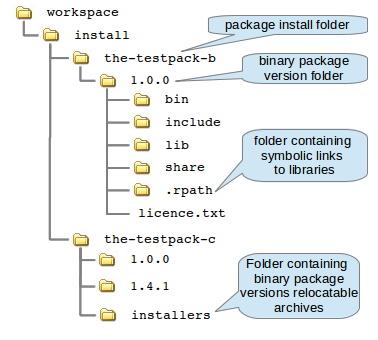
\includegraphics[scale=1]{images/installedBinaryPackage.png}
\caption{Example folder hierarchy for installed packages}
\label{fig:installBinaryFolder}
\end{figure}

Figure~\ref{fig:installBinaryFolder} provides an example of the workspace's install folder containing two installed packages. There can be many versions of the same package installed in the workspace as for the package "the-testpack-c", which has two versions installed. The \textbf{installers} folder for this later package may contains many binary package version relocatable archive (quickly called \textbf{package installer}), for instance two for each installed version. Indeed each binary version is associated with two \textbf{package installers}: one for \textit{Release} mode and one for \textit{Debug} mode. \textbf{Package installers} are zip archives (since cmake is able to compress and extract those archives in a cross-platform way) with following pattern for their name: <package name>-<package version number>-<operating system>[-dbg].zip. \textbf{Package installers} for \textit{Debug} mode have an additional "-dbg" postfix notation appended to their name.

Each binary package version folder also have a \texttt{.rpath} folder which is a PID specific folder used for configuring runtime links of PID components. It contains, for each binary executable component (share libraries binaries, applications binaries) of the package a set of symbolic links that points to the adequate shared libraries. PID system can reconfigure "on demand" run-time dependencies depending on the shared libraries versions installed and used. This system allows to create relocatable and reconfigurable binary code without using system mechanisms. Developers should never change the content of the \textbf{.rpath} folder "by hand", otherwise it could cause troubles.

\pagebreak

\section{Good practices}

\subsection{Structuring development with packages}

\subsubsection{Overview}

The basic guideline is to separate software into many packages that are structured according to a strict "depends" hierarchy as described in figure~\ref{fig:pack-hierarchy}. The "depends" relationship simply describes package dependencies as they are described in the CMakeList.txt of packages using the CMake PID function \texttt{declare\_PID\_Package\_Dependency} (see section~\ref{sec:rootCMakeDeps}). It just means that a source package requires another package to be installed in the workspace or in the system (for external packages). 

From a functional point of view a dependency can generally represent one of these two alternatives relationship:
\begin{itemize}
\item an \textbf{extension} relation : a child package \textbf{extends} a base package if it provides some \textit{functionalities} that specialize/extends those of the base package. This is a typical relationship when a library extends the class hierarchy provided by a library of the parent package, or/and when a more specialized/complete version of an application is provided.
\item a \textbf{use} relation : a child package \textbf{uses} a base package if it provides \textit{new functionalities} built onto those provided by the base package. This is the case when new libraries are using more basic ones or when new applications are built using existing components.
\end{itemize}

\begin{figure}
\center
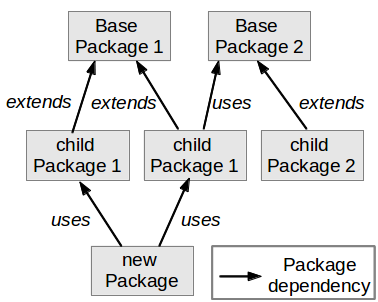
\includegraphics[scale=1]{images/package_hierarchy.png}
\caption{An example hierarchy of packages}
\label{fig:pack-hierarchy}
\end{figure}

\subsubsection{General guideline applied to packages}
\begin{itemize}
\item The names of packages \textbf{must be unique} considering all developed packages in the frame of the laboratory. Names are alphanumeric lower case ascii characters, without space but can include '-' for separating names in compound names.
\item \textbf{Cyclic dependencies between packages are forbidden}.
\item If a package has some dependencies induced by lower levels of the class hierarchy, prefer making a package for the higher level with less dependencies, and one or more dependent \textbf{extension} packages for the lower levels, each of them with the strict minimum required dependencies.
\item When developing a component for a given middleware (ROS, OROCOS, etc.) always put the functional code (library) in one package and extend this package each time a component is built from this code.
\item Dependencies to multiple packages are allowed but the developer should keep in mind to have the lowest possible number of dependencies for a given package, to keep relationship between packages understandable.
\item The number of \textbf{direct dependencies to external packages} should be very limited for a given package (0 to 5 max).
\item If possible, it is a better choice to choose a \textbf{commonly used external package} (e.g. boost, eigen, etc.) than a very specific one to define a dependency with a required external package.
\end{itemize}

\subsubsection{Guideline relative to developed functionalities}
\begin{itemize}
\item Try limiting the number of software artefacts generated by a package. Typical use is \textbf{one package per functionality}. For a given \textit{functionality}, the package defines :
\begin{itemize}
\item libraries implementing the functionality core behaviours and eventually example applications to explain how to use these libraries.
\item applications if this functionality can be directly used by end-users.
\item test units to control that all these libraries and components work well.
\end{itemize}
\item Different variations of a same \textit{functionality} should be developed in the same package. For instance if developers define many variations of a same library (e.g. typically static and shared version) that all implements the same \textit{functionality} (i.e. do the same thing from user point of view), each variation should be contained as a specific component in the same package. 
\item Components participating to the same \textit{functionality} should be developed in the same package. For instance if a set of application components (e.g. command line tools) are used to achieve a same objective, they should be developed in the same package. As a concrete example, the CMake command line tools suite could be developed in the same package.
\item Limit the number of hierarchical level to the strict necessary. As a global guideline we discourage having more than 4 hierarchical levels for the "extends" dependency to keep the extension hierarchy understandable.
\item A given package should only have an "extends" dependency with one package at maximum.
\end{itemize}

\subsection{Conventions}

This section explains good practices and guidelines when developing C/C++ code in PID packages.

\subsubsection{Files and folders naming convention}
\begin{itemize}
\item Package's folder names have the same name as the repository which is also the same name as the one declared in the CMakeList.txt file of the package (see section~\ref{sec:rootCMake}).
\item Sub-folders of package's standard folder (\textbf{src}, \textbf{include}, \textbf{apps}, \textbf{test}) are alphanumeric lower case ascii characters, without space but can include underscores ('\_') for separating names in compound names.
\item All executables and libraries names are alphanumeric sequence of lower case ascii characters words using only  '-' as special characters between each word.
\item C/C++ files' names are alphanumeric sequence of ascii lower case words using only underscores ('\_') as special characters between each word.
\item C++ source files have a .cpp or.cc extension , C source files have a .c extension. 
\item C++ header files  have a .h or.hh, C header files have a .h extension.
\item Template header files have a .hpp extension and template functions/ classes should always be entirely defined in header files, not in source files.
\item Files defining a C++ class have the name of the class. Only one class can be defined in a file (except internal classes).
\end{itemize}

\subsubsection{C/C++ objects naming convention}
\begin{itemize}
\item Classes/structures/enums/namespaces: their name is made of words, each word starting with a upper case character and other characters are lower case. Avoid too long names (e.g. \texttt{class FooBar} NOT \texttt{class TheClassFooBarIsAReallyLongNameForAClass}).
\item Names  of variables and functions' arguments are alphanumeric lower case sequence of words using only underscores ('\_') as special characters between each word (e.g. \texttt{int my\_variable\_name}).
\item Names of classes' attributes follows the same rule as variables but ends with an underscore (e.g. \texttt{int my\_attribute\_name\_}).
\item Constants are all capital, words are separated by underscores (e.g. const int MY\_CONSTANT).
\item Names of functions/methods have lower case characters except the first character of each word, but not for the first word that is full lowercase. Words are separated by underscores (e.g. \texttt{int this\_Is\_The\_Name\_Of\_ My\_Function(...)}).
\end{itemize}

\subsubsection{C/C++ coding guideline}
\begin{itemize}
\item \textbf{Indentation}: the indentation of the code should follow the bloc structure of the program. Put only one instruction by line.
\item \textbf{Comprehensive naming} : make your variables/functions/classes' names explicit and comprehensive as regard of the context. Use real life words, avoid meaningless random sequence of letters (e.g. one-letter names) except for integral iterator variables (i, j, k). An exception is tolerated if the notation come from a paper (e.g. matrix name).
\item \textbf{Package scoping}: use namespaces to scope your code and gather all classes, functions and global variables (e.g. constants) that belong to a same package. Each package as thus its own namespace whose name is the name of package (same words) but with namespace naming convention.
\item \textbf{Namespace inheritance}: when a package defines an "extends" dependency with another package, its namespace is prefixed with its parent package namespace (e.g. namespace \texttt{parent} for parent package namespace, namespace \texttt{parent::child} for the child package namespace).
\item \textbf{Class inheritance}: The basic usage is to subclass by using the public virtual statement (this  corresponds to the standard specialization mechanism when using multiple inheritance in object oriented programming. Never use protected or private inheritance. Use non virtual inheritance only if you are sure that  multiple inheritance will not take place in the hierarchy of the target class.
\item \textbf{Class protection}:  all attributes of a class must be \texttt{private} : define \texttt{public} or \texttt{protected} getters and/or setters only for attributes that can be accessed outside the class. Methods used only internally to a class must be \texttt{private}. Methods that are used in base class but that can be redefined in child classes must be\texttt{protected}. In a sub-class, never change the protection of elements defined in its base class.
\item \textbf{Friendship}: use \texttt{friend} statement with care: \texttt{friend} keyword should be used only if a class as specific access to a "private interface" (set of private or protected methods) of another class (the accessed class declares the accessing class as a friend). This is used when two classes in two distinct inheritance hierarchies are deeply bound to each other. 
\item \textbf{Polymorphism}: by default all \texttt{public} and \texttt{protected} methods must be \texttt{virtual}, and \texttt{private} methods have to be not \texttt{virtual}. If a \texttt{public} or \texttt{protected} method cannot be redefine in sub-classes then make them not \texttt{virtual} (e.g. most of time the case for getters/setters).
\item \textbf{Templates}: templates classes and functions must be completely defined in header files.
\item \textbf{Inlining}: never inline a \texttt{virtual} method ; inline only short methods that are to be widely used (getters and setters for example).
\item \textbf{Guarding headers}: the headers must be protected by multiple inclusion by using \texttt{\#ifndef} guards. Guards names follow constants naming convention with following structure : <package>\_<file name>\_H. For instance:
\begin{verbatim}
#ifndef PACKAGE_FILE_H 
#define PACKAGE_FILE_H 
...
#endif //PACKAGE_PATH_FILE_H 
\end{verbatim}
\item \textbf{Functions}: output arguments to methods/functions (i.e., variables that the function can modify) are passed by pointer, not by reference. Input "heavy objects" should be passed by const reference or pointer to \texttt{const} objects. For instance:
\begin{verbatim}
int example_Method(const Foo & in, Bar* out); 
int other_Method(const Foo * in, Bar* out);
\end{verbatim}
\item \textbf{Functions arguments}: limit the number of arguments of a function to 5 at maximum.
\item  \textbf{Be a const addict}: add \texttt{const} whenever it is possible: in the parameters of a function (input/output) and for methods that must not modify the class attributes. Return elements by \texttt{const} reference when you want to make readable an object attribute of a class or by pointer on \texttt{const} object when you want to make readable a pointer attribute.For instance:
\begin{verbatim}
const std::vector<double> & get_Attribute_Value() const;
const Bar * get_Attribute_Pointer() const;
\end{verbatim}
\item \textbf{Preprocessor macros and constants}: should be avoided. Prefer \texttt{inline} functions, \texttt{enums}, and \texttt{const} variables.
\item \textbf{Preprocessor instructions}: usage of \#ifndef, \#if, etc. should be limited as far as possible, except when dealing with platform specific code (OS specific libraries) or when dealing with alternatively available package dependencies (see section~\ref{sec:rootCMakeComplexDeps}).
\item \textbf{Exceptions}: exceptions are the preferred error-reporting mechanism for C++, as opposed to returning integer error codes. Always document what exceptions can be thrown by your package, on each function / method. Do not throw exceptions from destructors. Do not throw exceptions from callbacks that you do not invoke directly. When your code can be interrupted by exceptions, you must ensure that resources you hold will be deallocated when stack variables go out of scope. In particular, mutexes must be released, and heap-allocated memory must be freed. Accomplish this safety by using smart pointers.
\item \textbf{Documentation}: use doxygen annotations in header files to describe all methods (arguments, return value, usage, etc.), attributes, class (role and relationship with other classes), etc. These comments will be automatically included when the api documentation will be generated (see section~\ref{sec:apiCMakeHeaders}).
\item \textbf{Licensing}: systematically apply a license, authors and version information at the beginning of all source file (C/C++ headers and source). For license text, see the license cmake script file corresponding to the license used (it can be found in the workspace, see section~\ref{sec:workspace}).
\item \textbf{Threading}: avoid the management of multi-threading (processes/thread execution management, usage of IPC and synchronization mechanisms) into libraries and implement these mechanisms inside applications. Library should contain only computational code while applications embed control-flow management code. This rule is not valid for libraries, like those of middleware, implementing task management and communication mechanisms.
\end{itemize}

\pagebreak

\part*{Conclusion}

Concerning package development, developers have to refer to dedicated document explaining coding rules and general code development guidelines.

\pagebreak

\part*{Appendix}

\section{PID cmake functions API}
\label{sec:PIDCMakefunctionsAPI}

With PID there are few functions to use to precisely declare the content of a package. Each of these functions is detailed below. Note that optional arguments are signalled using the optional keyword into brackets.

\subsection{declare\_PID\_Package}

\textbf{Inputs argument}: 
\begin{itemize}
\item AUTHOR <name>. This is a string defining the name(s) of the reference author.
\item \{optional\} INSTITUTION <institutions>. This is a string defining the institutions to which the main author belongs.
\item YEAR <dates>. This is a string character that reflects the life time of the package, for instance "year of creation - year of last modification".
\item LICENSE <license name>. This is the name of the license applying to the package. This license name must be defined by a corresponding cmake file in the \textbf{licenses} directory of the workspace.
\item \{optional\} ADDRESS <url>. This argument represents the url of the package's git repository. It can be let undefined for pure local repository but must be set once the package is delivered.
\item DESCRIPTION <description>. This argument is a string that provides a short description of the package usage and utility.
\end{itemize}
\textbf{Constraints}: this function must be called in the root CMakeList.txt file of the package, before any other call to PID or \texttt{find\_package} (or equivalent) functions.\\
\textbf{Effect}: initialization of package's internal state.

\subsection{set\_PID\_Package\_Version}

\textbf{Inputs argument}:
\begin{itemize}
\item <major>. This is a positive digit indicating major version number.
\item <minor>. This is a positive digit indicating minor version number.
\item \{optional\} <patch>. This is a positive digit indicating patch version number. If not defined the patch version number of the package will be set to 0.
\end{itemize}
\textbf{Constraints}: this function must be called in the root CMakeList.txt file of the package, after \texttt{declare\_PID\_Package} and before \texttt{build\_PID\_package}.\\
\textbf{Effect}: set the current version number of the package. This will impact on the installed binary folder and configuration files.

\subsection{add\_PID\_Package\_Author}

\textbf{Inputs argument}: 
\begin{itemize}
\item AUTHOR <name>. This is a string defining the name(s) of an author of the package.
\item \{optional\} INSTITUTION <name>. This is a string defining the names of the institutions to which the author belongs.
\end{itemize}
\textbf{Constraints}: this function must be called in the root CMakeList.txt file of the package, after \texttt{declare\_PID\_Package} and before \texttt{build\_PID\_package}.\\
\textbf{Effect}: add another author to the list of authors of the package.

\subsection{add\_PID\_Package\_Reference}
\label{sec:PIDCMakefunctionsAPI_add_reference}
\textbf{Inputs argument}:  2 signatures whether the user wants to add a binary package reference or to shadow the official git repository address.
\begin{itemize}
\item SOURCE option is used when user wants to shadow the official source repository address.
\begin{itemize}
\item URL <address>. This argument specifies the address of the \textbf{private git repository} to use instead of the official address.
\end{itemize}
\item BINARY option is used to add a reference to a binary package version.
\begin{itemize}
\item VERSION <major> <minor> \{optional\}<patch>. This argument describes the full version number of the referenced binary package. <major> <minor> and <patch> are positive digits. If patch number is omitted then patch number is considered as 0.
\item SYSTEM <name>. This is the name of the target operating system. For now only linux supported.
\item URL <url-rel> <url-dbg>. The two values of the URL arguments are: the url of the package binary in release version and the url of the package binary in debug version.
\end{itemize}
\end{itemize}

\textbf{Constraints}: this function must be called in the root CMakeList.txt file of the package, after \texttt{declare\_PID\_Package} and before \texttt{build\_PID\_package}.\\
\textbf{Effect}: reference addresses where to find a given binary package version for a given operating system. This information will be used to generate a CMake configuration file that will be used for retrieving adequate package versions.

\subsection{declare\_PID\_Package\_Dependency}
\textbf{Inputs argument}: 2 signatures whether the dependency is an external or a PID package.
\begin{itemize}
\item For external packages:
\begin{itemize}
\item PACKAGE <name>. The string without white space defining the unique identifier of the required external package.
\item EXTERNAL <path>. This is the path to the root directory of the external package. This path will be used as the basic reference for any folder/component of the external package that is referenced by local components.
\item \{optional\} VERSION <version string>. This version is a string without white space and following dotted notation of versions, that indicates which version of the external package is required.
\end{itemize}
\item For PID packages:
\begin{itemize}
\item PACKAGE <name>. The string without white space defining the unique identifier of the required PID package.
\item PID. This option is just used to indicates that the required package is a PID package.
\item \{optional\} VERSION <major> <minor>. Major and minor version number are positive digits that are used to constraint the required package to a given version.
\item \{optional\} EXACT. This option is used only if the VERSION argument is used. It indicates that the required package version is exactly the major.minor version required. Patch version is let undetermined.
\item \{optional\} COMPONENTS <list of components>. This argument is used to specify which components of the required package will be used by local components. If not specified there will be no check for the presence of specific components in the required package.
\end{itemize}
\end{itemize}
\textbf{Constraints}: this function must be called in the root CMakeList.txt file of the package, after \texttt{declare\_PID\_Package}, after the \texttt{find\_package} call to the same required package and before \texttt{build\_PID\_package}.\\
\textbf{Effect}: this function will register the target package as a dependency of the current package. These informations will be useful to generate adequate configuration files for the current package. Each required package \textbf{MUST BE referenced} using this function.

\subsection{build\_PID\_Package}
\textbf{Inputs argument}: none.\\
\textbf{Constraints}: this function must be the last one called in the root CMakeList.txt file of the package.\\
\textbf{Effect}: this function generates configuration files, manage the generation of the global build/install process and will call CMakeList.txt files of the following folders: \textbf{src}, \textbf{apps}, \textbf{test}, \textbf{share}.

\subsection{declare\_PID\_Component}
\textbf{Inputs argument}:
\begin{itemize}
\item <type>. This argument specifies the the type of the component. Its value is either STATIC\_LIB (static library), SHARED\_LIB(shared library), HEADER\_LIB (header library), APPLICATION (stadard applciation),EXAMPLE\_APPLICATION (example code), TEST\_APPLICATION (test unit)
\item NAME <name>. This is the string without white space defining the unique identifier of the component.
\item DIRECTORY <dir>. This is the directory where to find component source. Depending on its <type> this directory is a sub-folder of the \textbf{src} (library), \textbf{apps} (example or standard application) or \textbf{test} (test unit) package's folders.
\item \{optional\} INTERNAL. This argument is followed by other arguments that are only local to the component, i.e. that it does not export.
\begin{itemize}
\item \{optional\} DEFINITIONS <defs>. These are the preprocessor definitions internally used by the component's source code. For libraries these definitions must not be part of one of their header files. This is used to provide a given implementation to the component among different alternative, for instance to match operating system requirements.
\item \{optional\} INCLUDE\_DIRS <dirs>. These are additional directory where to find header files (that are not part of their interface for libraries).
\item \{optional\} LINKS <links>. These are link flags, like path to lirabries. This argument is used mainly by applications.
\end{itemize}
\item \{optional\} EXPORTED\_DEFINITIONS <defs>. These are the preprocessor definitions that are contained in one or more of libraries header files. Applications do not export any definition.
\end{itemize}
\textbf{Constraints}: Depending of the <type> of the component this function must be called in the adequate CMakeList.txt file (either in the \textbf{src}, \textbf{apps} or \textbf{test} folders. It must be called before any call to declare\_PID\_Component\_Dependency applied to the same declared component\\
\textbf{Effect}: this function is used to define a component in the current package. This will create adequate targets to build the component binary (if any) and install it.

\subsection{declare\_PID\_Component\_Dependency}
\textbf{Inputs argument}:2 signatures whether the dependency is an external or a PID package. 
\begin{itemize}
\item common arguments for both signature:
\begin{itemize}
\item COMPONENT <name>. This is the string without white space that defines the local component for which a dependency is defined.
\item \{optional\} EXPORT. This is an option indicating if the component <name> exports the required dependency. Exporting means that the reference to the dependency is contained in its interface (header files). This can be only the case for libraries, not for applications.
\item \{optional\} INTERNAL\_DEFINITIONS <defs>. These are preprocessor definitions used internally to the component source code, when using the dependency. The definitions must not be part of the component header files (they are never exported).
\item \{optional\} IMPORTED\_DEFINITIONS <defs>. These are preprocessor definitions \textbf{contained in the interface (header files) of the dependency} that are set (or unset) when the component use this dependency.
\item \{optional\} EXPORTED\_DEFINITIONS <defs>. These are preprocessor definitions \textbf{contained in the interface (header files) of the component} that are set or unset anytime when this component will be used.
\end{itemize}
\item for a required PID component:
\begin{itemize}
\item DEPEND <dep\_component>. This is the specification of the dependency. In this case the dependency is a required PID component and <dep\_component> is simply the name of this component.
\item \{optional\} PACKAGE <dep\_package>. If the PACKAGE argument is used, it means that the required component belongs to another package. In this case, <dep\_package> is the name of the required package, which must have been declared as a package dependency before (in the root CMakeList.txt file of the package). If PACKAGE argument is not used, it means that the required component is part of the current package.
\end{itemize}
\item for a required external component, the dependency can target either a system dependency or a custom external dependency:
\begin{itemize}
\item \{optional\} EXTERNAL <ext\_package> INCLUDE\_DIRS <dirs>. When EXTERNAL argument is used, it means that the dependency is over a custom external package. In such a case <ext\_package> is the name of the external package which must have been declared as a package dependency (in the root CMakeList.txt file of the package). The argument INCLUDE\_DIRS is then used to specify where to find headers of the libraries used, <dirs> being the list of path to these includes, relative to the package root dir.
\item \{optional\} LINKS. This is an option to specify target libraries used. If used, then there must be STATIC and/or SHARED arguments used.
\item STATIC <links>. These are the static libraries used. For system libraries, system referencing must be used (e.g. -lm for libm.a). For custom external packages complete path to libraries, relative to required external package root dir must be used.
\item SHARED <links>. These are the shared libraries used. For system libraries, system referencing must be used (e.g. -lm for libm.so). For custom external packages, complete path to libraries, relative to required external package root dir must be used.
\end{itemize}
\end{itemize}
\textbf{Constraints}: Depending of the <type> of the component this function must be called in the adequate CMakeList.txt file (either in the \textbf{src}, \textbf{apps} or \textbf{test} folders. It must be called after the call to declare\_PID\_Component applied to the same declared component\\
\textbf{Effect}: this function is used to define a dependency between a component in the current package and another component (headers, static or shared library), either an external component or a PID component. This will configure the build process for the component binary (if any).

\pagebreak

\section{Examples}
\label{sec:Examples}

\subsection{Package the-testpack-b}

\subsubsection{Root CMakeList.txt}

\begin{verbatim}
PROJECT(the-testpack-b)
CMAKE_MINIMUM_REQUIRED(VERSION 2.8.11)
set(WORKSPACE_DIR ${CMAKE_SOURCE_DIR}/../.. 
	CACHE PATH "root of the packages workspace directory")
list(APPEND CMAKE_MODULE_PATH ${WORKSPACE_DIR}/share/cmake/system)
include(Package_Definition)

declare_PID_Package(	
   AUTHOR       Robin Passama 
   INSTITUTION  LIRMM 
   YEAR         2013 
   LICENSE      CeCILL
   ADDRESS      git@idh.lirmm.fr:perso/passama/the-testpack-b.git
   DESCRIPTION  test package B for PID
)

set_PID_Package_Version(1 1)

# adding some binary packages references
add_PID_Package_Reference(	
     BINARY VERSION 0 1 0 SYSTEM linux URL 	
http://lirmm.lirmm.fr/FileX/get?auto=1&k=rfYTf1gkpI5XtEpQWVA
http://lirmm.lirmm.fr/FileX/get?auto=1&k=oMyg4JVeeKYWpqwEFxE)

add_PID_Package_Reference(
     BINARY VERSION 1 1 SYSTEM linux URL 	
http://lirmm.lirmm.fr/FileX/get?auto=1&k=DYt2j35Kw8ozOgHfoVA
http://lirmm.lirmm.fr/FileX/get?auto=1&k=zEx02N4KWfzDWPTxiO)


# from here we manage packages dependencies #
find_package (Boost REQUIRED) #system library
find_package (the-testpack-a 1.0 REQUIRED lib-b-sh lib-x)

if(NOT Boost_FOUND)
   message("FATAL_ERROR Boost has not been found 
            -> impossible to build ${PROJECT_NAME} package")
	return()
endif()

if(Boost_DIR-NOTFOUND)
	set(BOOST_ROOT /usr)
endif()

declare_PID_Package_Dependency(
    PACKAGE Boost 
    EXTERNAL ${BOOST_ROOT} 
    VERSION "${Boost_MAJOR_VERSION}.${Boost_MINOR_VERSION}.
${Boost_SUBMINOR_VERSION}")

declare_PID_Package_Dependency (
   PACKAGE the-testpack-a
   PID VERSION 1 0 
   COMPONENTS lib-b-sh lib-x)

build_PID_Package()

\end{verbatim}

The package the-testpack-b (version 1.1) requires the Boost external package and the package the-testpack-a (version 1.0). It defines URL where to find binary package version relocatable archive using the \texttt{add\_PID\_Package\_Reference} function.

\subsubsection{Libraries}

Libraries source code is contained in \textbf{include} and \textbf{src} sub-folders of the package. The CMakeList.txt file of the \textbf{src} folder declare available libraries:

\begin{verbatim}
#libY -> dependency with libX
declare_PID_Component(HEADER_LIB NAME lib-y DIRECTORY lib_y)
declare_PID_Component_Dependency (COMPONENT lib-y EXPORT 
DEPEND lib-x PACKAGE the-testpack-a
EXPORTED_DEFINITIONS USE_EXTERNAL_LIB_X)

#libYBis -> dependency with libX
declare_PID_Component(HEADER_LIB NAME lib-y-bis DIRECTORY lib_y
EXPORTED_DEFINITIONS NUSE_EXTERNAL_LIB_X)

#libC shared -> dependency with libY
declare_PID_Component(SHARED_LIB NAME lib-c-sh DIRECTORY lib_c
INTERNAL DEFINITIONS A_VERY_SPECIFIC_IMPLEM)
declare_PID_Component_Dependency(COMPONENT lib-c-sh EXTERNAL Boost 
INCLUDE_DIRS <Boost>/include)
declare_PID_Component_Dependency(COMPONENT lib-c-sh EXPORT 
DEPEND lib-y)


#libC static -> dependency with libY
declare_PID_Component(STATIC_LIB NAME lib-c-st DIRECTORY lib_c
INTERNAL	 DEFINITIONS NA_VERY_SPECIFIC_IMPLEM)
declare_PID_Component_Dependency(COMPONENT lib-c-st EXTERNAL Boost 
INCLUDE_DIRS <Boost>/include)
declare_PID_Component_Dependency(COMPONENT lib-c-st EXPORT 
DEPEND lib-y-bis)
\end{verbatim}

The declared libraries are:
\begin{itemize}
\item \textit{lib-y} a header library, whose header files are in the \textbf{lib\_y} sub-folder of the \textbf{include} folder.
\item \textit{lib-y-bis} a header library, whose header files are the same as those of \textit{lib-y} (same folder used), but whose definitions used are different (thus modifying the behaviour of the library).
\item \textit{lib-c-sh} a shared library, whose header files are in the \textbf{lib\_c} sub-folder of the \textbf{include} folder, and whose source files are in the \textbf{lib\_c} sub-folder of the \textbf{src} folder.
\item \textit{lib-c-st} a static library based on the same source code that the \textit{lib-c-sh} library (same folders) but with different definitions and dependencies and built a different way (as an archive instead of a dynamic object).
\end{itemize}

\paragraph{shared code between lib-y and lib-y-bis libraries}
The folder \texttt{<package root>/include/lib\_y} contains a header file named \textit{libY.h} whose content is: 
\begin{verbatim}
#ifndef LIBY_INCLUDE
#define LIBY_INCLUDE
#include <stdio.h>

#ifdef USE_EXTERNAL_LIB_X
#include <libX.h>
typedef struct{
    LibXType onetwo;
    unsigned char three; char four;
    unsigned long five;
} LibYType;
#else
typedef struct{
    char tutu [256];
    unsigned char tata[12];
    unsigned char three;
    char four; unsigned long five;
} LibYType;
#endif

typedef LibYType YBuffer[10];
void liby_print(YBuffer yb){
    for (unsigned int i = 0; i < 10;i++){
#ifdef USE_EXTERNAL_LIB_X
    #ifdef USE_LIBX_PRINT
        libx_print(yb[i].onetwo);
    #else 
        #ifdef USE_LIBA_FOR_COMPUTING
        libx_print_with_liba(&yb[i].onetwo);
        #else
           #error "NO IMPLEMENTATION AVAILABLE FOR LIBX !!!"
        #endif
     #endif
	     printf("three : %d, four = %c, five : %lu\n", 
	     yb[i].three, yb[i].four, yb[i].five);
#else
    printf("tutu : %s, tata : %s, three : %d, four = %c, 
    five : %lu\n", yb[i].tutu, yb[i].tata, yb[i].three, 
    yb[i].four, yb[i].five);
#endif
    }
}
#endif
\end{verbatim}
As reader can notice, depending on the value of the \texttt{USE\_EXTERNAL\_LIB\_X} preprocessor variable, this code will have different behaviours. It will notably condition the use of another library \textit{lib-x} supposed to be defined in another package, because it condition the \texttt{\#include<libX.h>} directive. In CMakeList.txt, the \textit{lib-y} header library component defines this preprocessor variable while the \textit{lib-y-bis} header library component undefines it:
\begin{itemize}
\item when \texttt{USE\_EXTERNAL\_LIB\_X} is defined it forces the use of a dependency to another component \textit{lib-x} of another package \textit{the-testpack-a}. When this dependency is declared the \texttt{EXPORTED\_DEFINITION} keyword is used to say that the preprocessor variable is defined in the interface (a header file) of \textit{lib-y}. In this case the \textit{lib-x} component is exported (use of \texttt{EXPORT} keyword in dependency declaration) since it is contained in the interface (a header file) of the \textit{lib-y} component.
\item  when \texttt{USE\_EXTERNAL\_LIB\_X} is not defined (using \texttt{NUSE\_EXTERNAL\_LIB\_X} to negate it) the dependency to lib-x component is not defined (no \texttt{\#include<libX.h>} directive). Consequently the \texttt{EXPORTED\_DEFINITION} keyword is used directly into the \texttt{declare\_PID\_Component} function (see declaration of \textit{lib-y-bis}). Indeed, this preprocessor definition cannot be attached to a particular dependency (no dependency declared for \textit{lib-y-bis}).
\end{itemize}
This way we can associate different component to the same source code by playing on preprocessor variables. since these definition are exported they can be used by libraries that are using either version of this code (\textit{lib-y} or \textit{lib-y-bis}). For instance, we suppose that the \textit{lib-x} library also exports some preprocessor variable definitions, the same way as \textit{lib-y}: \texttt{USE\_LIBX\_PRINT} and \texttt{USE\_LIBA\_FOR\_COMPUTING}. The behaviour of \textit{lib-y} is conditional whether the preprocessor variable of \textit{lib-x} that has been defined by the component.

\paragraph{shared code between lib-c-sh and lib-c-st libraries}
The \texttt{<package root>/include/lib\_c} folder contains a header file named \textit{libC.h} whose content is: 
\begin{verbatim}
#ifndef LIBC_INCLUDE
#define LIBC_INCLUDE

#define LIB_C_CONST_VALUE 10.0256
extern "C"{
#include <libY.h> 
}
void libc_function1(YBuffer);
void libc_function2(YBuffer);

#endif
\end{verbatim}
The folder \texttt{<package root>/src/lib\_c} contains a source file named \textit{code1.cc} whose content is: 
\begin{verbatim}

#include <libC.h>
#include <stdio.h>
#include <boost/math/special_functions/factorials.hpp>

void libc_function1(YBuffer data){
    liby_print(data);
    double res = boost::math::factorial<double>(data[0].five);
    printf("factorial = %lf, with factor = %lf\n", res, 
            res*LIB_C_CONST_VALUE);
}

void libc_function2(YBuffer data){
#ifdef A_VERY_SPECIFIC_IMPLEM
    printf("SPECIFIC libc_function2 !!!\n");
    liby_print(data);
#else
    printf("STANDARD libc_function2 !!!\n");
    liby_print(data);
#endif
}
\end{verbatim}

As readers can notice the interface (header files) is the same for both libraries \textit{lib-c-sh} and \textit{lib-c-st}: there is no use of a  preprocessor variable in \textit{libC.h} to differentiate alternative signatures. Apart from the nature of their resulting binary (archive of objects or dynamic object) their main difference is an alternative implementation of the function \texttt{libc\_function2}, using preprocessor variable \texttt{A\_VERY\_SPECIFIC\_IMPLEM} (in \textit{code1.cc}). This variable is defined by \textit{lib-c-sh} and undefined by \textit{lib-c-st} with the \texttt{INTERNAL} keyword (see CMakeList.txt) since it applies only to the implementation of both component, not their interface (otherwise it would be defined with the \texttt{EXPORTED\_DEFINITION} keyword, like for \textit{lib-y} and \textit{lib-y-bis}). 

Both libraries have a dependency with the external Boost package (they need to know where are the include folders of that package) and they each define an internal dependency:
\begin{itemize}
\item \textit{lib-c-sh} depends on \textit{lib-y}, consequently \texttt{USE\_EXTERNAL\_LIB\_X} will be defined (by transitivity).
\item \textit{lib-c-st} depends on \textit{lib-y-bis}, consequently \texttt{USE\_EXTERNAL\_LIB\_X} will be undefined (by transitivity).
\end{itemize}
Finally both libraries will have slightly different behaviours depending on either (1) their local implementation and (2) their dependencies.

Finally readers can also notice that dependencies are exported or not:
\begin{itemize}
\item Dependency to external Boost package is not exported since the \texttt{\#include <boost/math/special\_functions/factorials.hpp>} directive is only in the \textit{code1.cc} source file.
\item Dependencies to \textit{lib-y} or \textit{lib-y-bis} are exported since the \texttt{\#include <libY.h>} directive is in the interface (\textit{libC.h}) of both libraries.
\end{itemize}

\subsubsection{Applications}




\pagebreak

\part*{POUBELLE}


 The workspace also provides categories : each category defines a specific subject that helps classifying packages/frameworks. For instance the category sensor will reference all packages or frameworks that implement the driver of a sensor. Categories can be hierarchically refined into sub categories for instance the category camera refines the category sensors. Categories can be viewed as lists of links that target frameworks/packages. The process of classification of packages is itself coming from package description (i.e. a package specifies the categories it belongs to).
 
the \textbf{categories} folder is structured according a set of topics, each topic being itself a folder that in turn contains either other subcategories or \textbf{links to frameworks}. \textbf{categories} only goal is to help finding available packages (under binary form) according to a given theme. Considering a category, packages that are relevant for the theme it defines are referenced as links (symbolic relative links in Linux) to frameworks folders.


\subsection{Licensing packages}

The licensing of packages has to be done according to a general politics of the laboratory, team or sub-group. License is let free to their decision and constraints, nevertheless, as software licenses are the same for everybody, licenses definitions are shared between all people.

The \textbf{licenses} folder contains definitions for all licenses that are available for use in package description. Each license is defined in a specific file that looks like this for the GPLv3 license (file name is "GNUGPLv3.license") :


\subsection{Categorizing packages}

When developing it is often useful to know which package provide some useful things relative to one or more topics. The aim of the \textbf{categories} folder is to standardize the classification and the finding of packages relevant for given concerns.

The \textbf{categories} folder is structured into subfolders that describe known categories. Each category folder is itself structured the following way:
\begin{itemize}
\item sub folder describes sub categories. A sub category refines the topic of its containing category. For instance folders \textbf{arms} and \textbf{wheeled vehicles} are contained in the category folder \textbf{robot}. These sub categories can in turn be refined the same way.
\item symbolic links represent target packages of the category. The name of the link is simply the name of the package, the target of the link is a given package framework. The target itself is always expressed as a \textbf{relative path} from the containing category folder to the target framework. By default these links target nothing in the file system as long as the package's framework has not been installed in the \textbf{frameworks} folder.
\end{itemize}

\paragraph*{Remark:} 
a same package can be targeted by more than one link: it means that the package belongs to different (sub)categories according to the different point of view of the developers. Doing so, anyone can have his own point of view of the package depending on its center of interest.
\linebreak

To organize the development, defining some "standard categories" should help developers to classify their packages. This requires to list categories of code that is useful for robotic applications development. For instance :
\begin{itemize}
\item sensors
\begin{itemize}
\item vision
\begin{itemize}
\item cameras
\item kinects
\item lasers
\end{itemize}
\item force sensors
\item encoders
\end{itemize}
\item robots
\begin{itemize}
\item arms
\item wheeled vehicles
\item humanoids
\end{itemize}
\item simulators
\item navigation
\begin{itemize}
\item cartography
\item positioning
\end{itemize}
\item planning
\begin{itemize}
\item mission
\item path
\item trajectory
\end{itemize}
\item middleware
\begin{itemize}
\item ros
\item contract
\item orocos
\end{itemize}
\end{itemize}

Of course categories can evolve/change along time, when developers want new categories.

\subsubsection{Working with categories}

The only people that can modify \textbf{categories} folder are package administrators. Each time a new package is created, developers define which are its relevant categories and wrote them in the package.manifest file of the package. When an administrator of a package wants to reference it :
\begin{itemize}
\item he first copy/rename the package.manifest file into the \textbf{references} folder.
\item according to the relevant categories of tha package defined in the manifest, he:
\begin{itemize}
\item creates new (sub)category folders in the the \textbf{categories} folder of its workspace, if the corresponding categories do not exist.
\item creates as many symbolic links that target the package framework as there are relevant categories for the package and put these links into the adequate category folders.
\end{itemize}
\item once done he commits its workspace.
\end{itemize}

From developers point of view, categories just help finding packages that are relevant for given topics. Each time they update their workspace, all available categories and classification of packages according to categories are updated. 

To search packages, they can simply navigate in the file system of the \textbf{categories} folder. 
\begin{itemize}
\item if the package is already installed in the \textbf{frameworks} folder he can simply follow the link.
\item otherwise the link is broken, and the developer has to install the corresponding package.
\end{itemize}

\end{document}